\pdfminorversion=4
% utf-8
\documentclass[notes=hide]{beamer}
\usepackage[utf8]{inputenc}
\usepackage[english]{babel}
\usepackage{graphicx}
\usepackage{wasysym}
\usepackage{alltt}
\usepackage{bbm}
\usepackage{stmaryrd}
\usepackage{eurosym}
\usepackage{amssymb}
\usetheme{uds}
\usepackage[dvipsnames]{xcolor}

\defbeamertemplate{headline}{page number}{%
	\vskip1pt%
	\setbeamertemplate{footline}[frame number]%
	\usebeamertemplate{footline}%
}

\setbeamertemplate{headline}[page number]
\setbeamerfont{smallfont}{size=\small}
\setbeamerfont{smallerfont}{size=\footnotesize}
\setbeamerfont{smallestfont}{size=\scriptsize}
\setbeamerfont{tinyfont}{size=\tiny}
\setbeamerfont{largefont}{size=\large}
\setbeamerfont{Largefont}{size=\LARGE}
%\setbeamerfont{page number in head/foot}{size=\tiny}
%\setbeamertemplate{headline}[frame number]


\newcommand\bluebox[2][uds@main]{{%
  \setlength{\fboxsep}{0pt}%
  \colorbox{#1}{#2\strut}%
}}

\def\Prob{\mbox{\bf P}}
\newcommand{\OO}{\mathcal{O}}
\newcommand{\N}{\mathbbm{N}}
\newcommand{\R}{\mathbbm{R}}
\newcommand{\len}[1]{{\vert #1 \vert}}
\newcommand{\emptystring}{\varepsilon}
\newcommand{\substr}[3]{#1[#2\ldots#3]}
\newcommand{\suffix}[2]{{#1}[{#2}\ldots]}
\newcommand{\prefix}[2]{{#1}[\ldots{#2}]}
\newcommand{\chr}[2]{#1[#2]}
\newcommand{\powset}[1]{2^{#1}}
\newcommand{\pos}{\ensuremath{\texttt{\upshape pos}}}
\newcommand{\lcp}{\ensuremath{\texttt{\upshape lcp}}}
\newcommand{\cld}{\ensuremath{\texttt{\upshape cld}}}
\newcommand{\rank}{\ensuremath{\texttt{\upshape rank}}}
\newcommand{\bwt}{\ensuremath{\texttt{\upshape bwt}}}
\newcommand{\bwtfind}{\ensuremath{\texttt{\upshape bwtfind}}}
\newcommand{\Occ}{\ensuremath{\texttt{\upshape Occ}}}
\newcommand{\less}{\ensuremath{\texttt{\upshape less}}}
\newcommand{\type}{\ensuremath{\texttt{\upshape type}}}
\newcommand{\lcpskip}{\ensuremath{\texttt{\upshape skip}}}
\newcommand{\gap}{\ensuremath{\text{--}}}
\newcommand{\iverl}{\llbracket}
\newcommand{\iverr}{\rrbracket}
\newcommand{\C}{\ensuremath{\texttt{\upshape C}}}
\newcommand{\T}{\mathcal{T}}
\newcommand{\I}{\mathcal{I}}
\newcommand{\F}{\mathcal{F}}
\newcommand{\X}{\mathcal{X}}
\newcommand{\A}{\mathcal{A}}
\newcommand{\RR}{\mathbb{N}}
\newcommand{\NN}{\mathbb{R}}
\newcommand{\W}{\mathcal{W}}

\newcommand{\blackboard}[1]{
\begin{block}<#1>{}
\begin{center}
\textbf{BLACK BOARD EXAMPLE}
\end{center}
\end{block}
}

\usepackage{listings} % ab Version 1.4 mit Python-Syntax-Highlighting!
\definecolor{mygray}{gray}{.50}
\lstset{language=Python,
    basicstyle=\scriptsize\ttfamily,
    stringstyle=\ttfamily\color{green},
    keywordstyle=\color{blue}\bfseries,
    commentstyle=\color{mygray},
    tabsize=4,
    numbers=left,
    numberstyle=\tiny,
    numbersep=5pt,
    morekeywords=assert,
    extendedchars=false,
    showstringspaces=false,
    frame=single
    }
\lstset{escapeinside={/*@}{@*/}}

\newcommand{\captionslide}[1]{
\begin{frame}
\frametitle{\phantom{NONE}}
\begin{center}
\vspace{1cm}
\usebeamerfont{Largefont}
          {\bf\em #1}
          \vspace{2cm}
\end{center}
\end{frame}
}
              
\title[Haplotype Assembly]{Read-Based Phasing of Related Individuals}
%\author[SG]{\textit{Shilpa Garg}\\ PhD Student, MPI-Inf, Saarbrücken, Germany \\with \\
%	Marcel Martin, Tobias Marschall }

\author[S.~Garg, M.~Martin, T.~Marschall]{\textcolor{blue}{Shilpa Garg~$^{1,2,3}$}, Marcel Martin~$^{4}$ and Tobias Marschall~$^{1,2}$}
\date{July 11, 2016}
\institute{\scriptsize $^{1}$Max Planck Institute for Informatics, Germany\\ $^{2}$Center for Bioinformatics, Saarland University, Germany \\ $^{3}$ Saarbr\"ucken Graduate School of Computer Science, Germany \\$^{4}$ Science for Life Laboratory, Dept. of Biochemistry and Biophysics, Stockholm University, Sweden}


\begin{document}

\frame[plain]{\titlepage}

\begin{frame}{What is Haplotyping/Phasing?}
\begin{center}
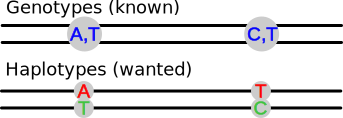
\includegraphics[width=.8\textwidth]{figs/diploid-phasing-no-reads}
\end{center}
\begin{block}<2>{Applications}
\begin{itemize}
	\item Personalized medicine
	\item Human migration, evolutionary selection and population structure
\end{itemize}
\end{block}
\end{frame}

\begin{frame}{Approaches to Phasing}
\begin{center}
\only<1>{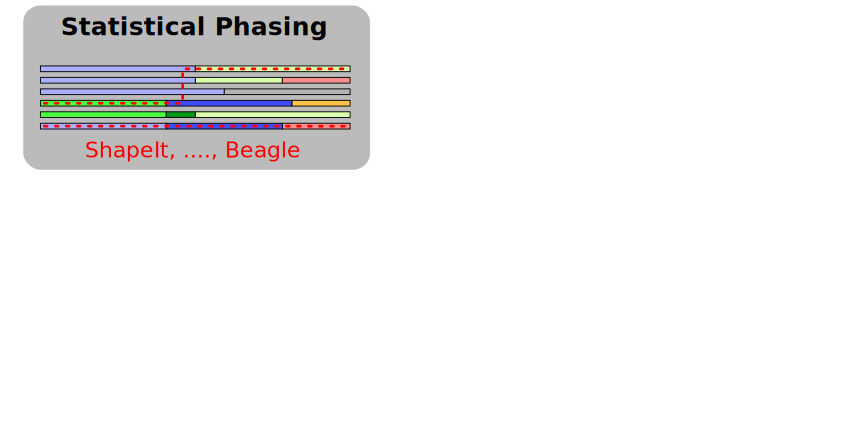
\includegraphics[width=\textwidth]{figs/haplotyping-overview1}}%
\only<2>{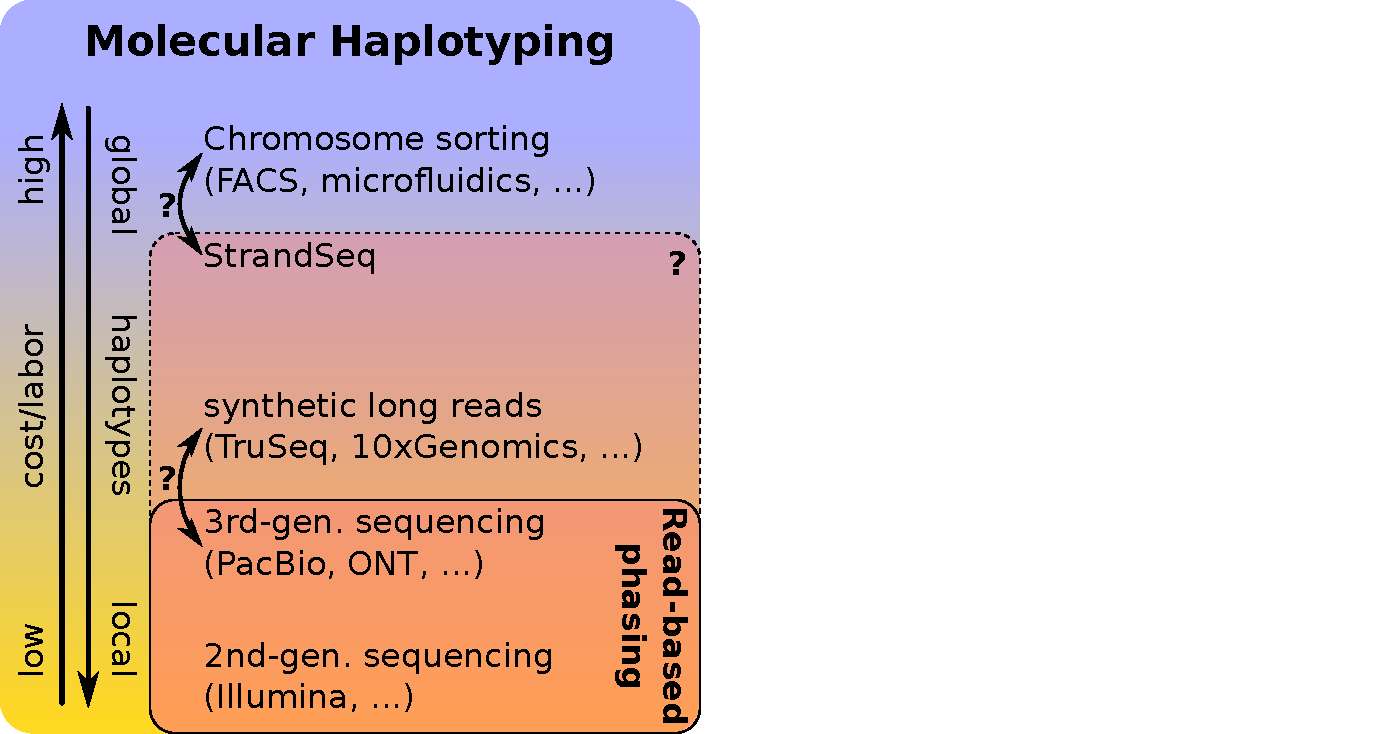
\includegraphics[width=\textwidth]{figs/haplotyping-overview2}}%
\only<3>{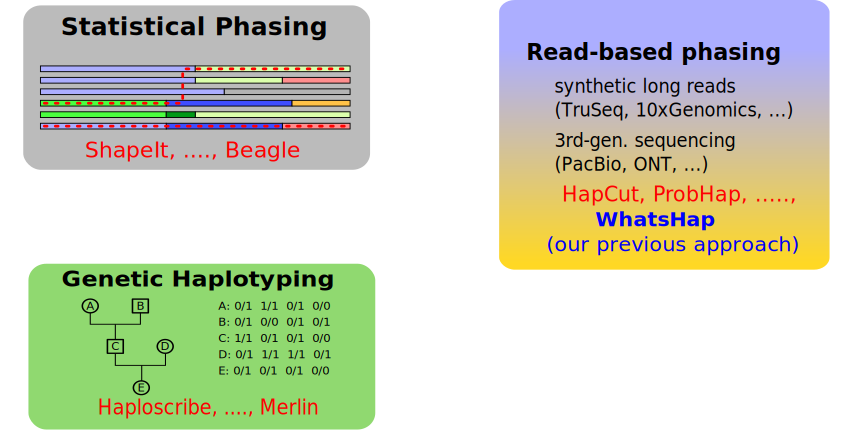
\includegraphics[width=\textwidth]{figs/haplotyping-overview3}}%
\only<4>{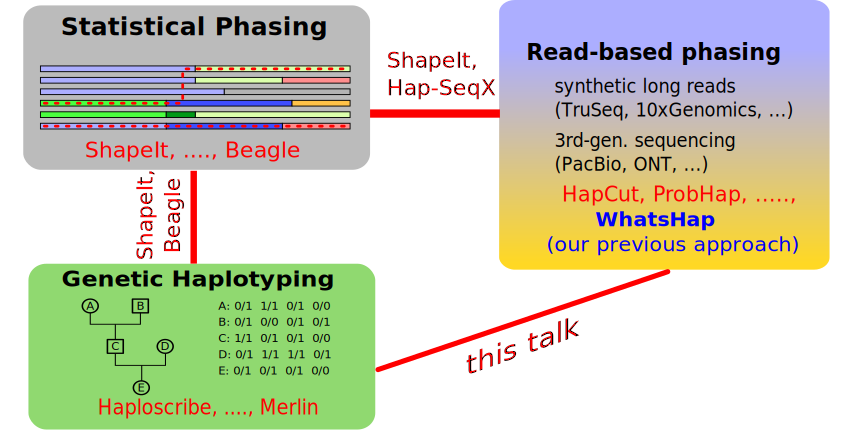
\includegraphics[width=\textwidth]{figs/haplotyping-overview4}}%

\end{center}
\end{frame}

\begin{frame}{Read-Based Phasing (Single Individual)}
\begin{center}
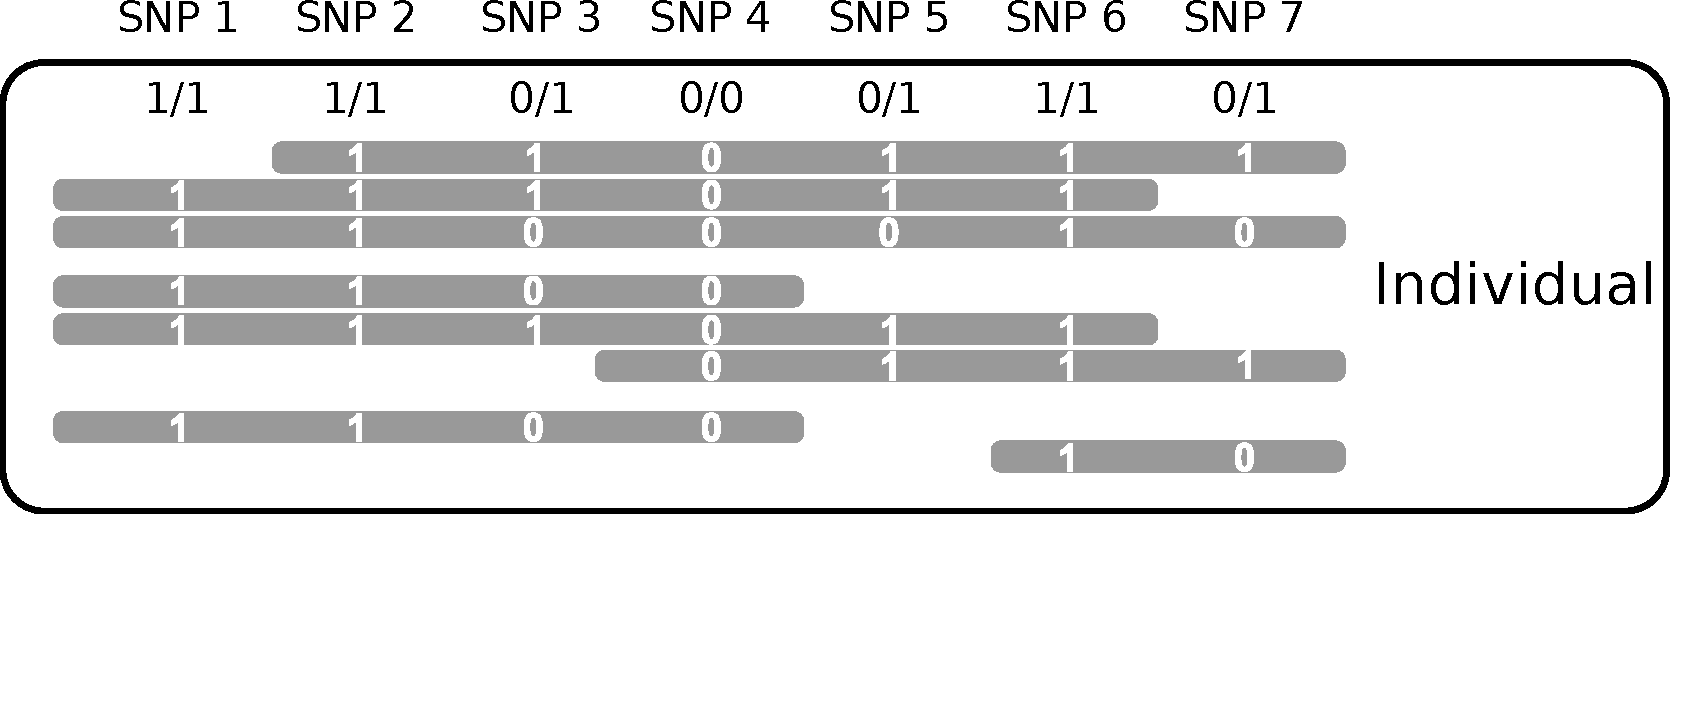
\includegraphics[scale=.35]{figs/sih-phasing-complete1.pdf}
\end{center}
\end{frame}

\begin{frame}{Read-Based Phasing (Single Individual)}
	\begin{center}
	%	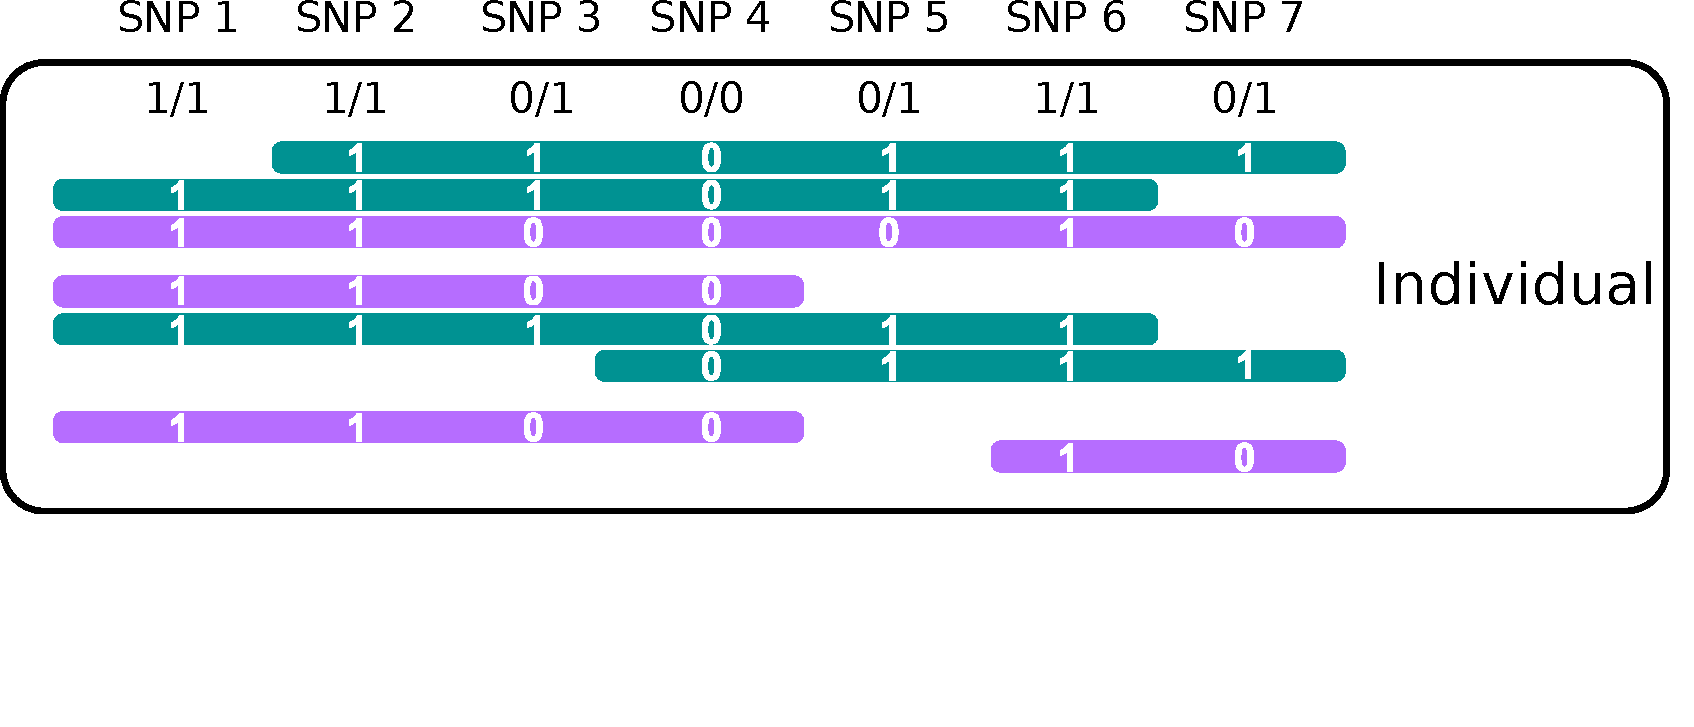
\includegraphics[scale=.3]{figs/sih-phasing-complete.pdf}
		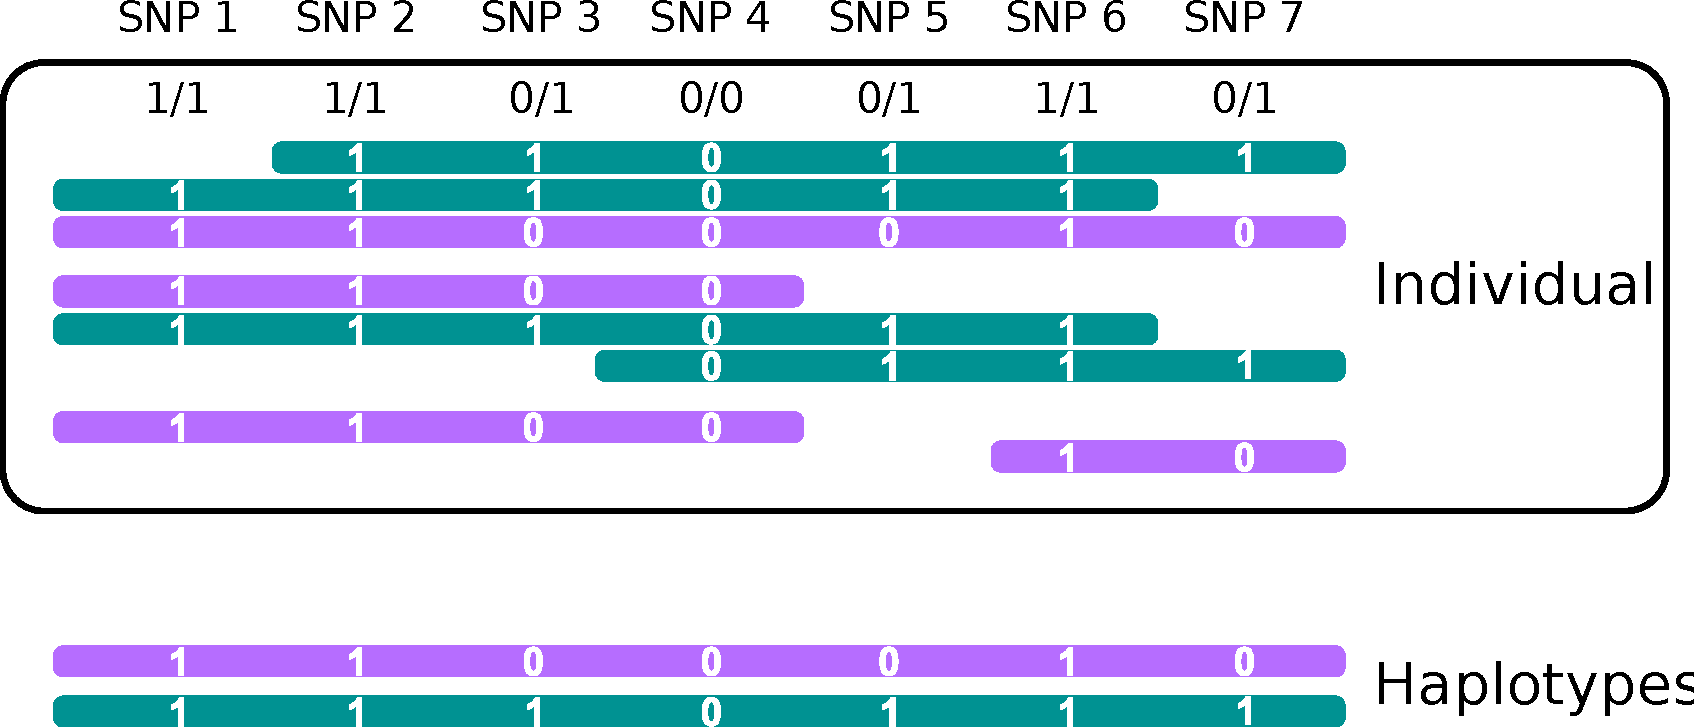
\includegraphics[scale=.35]{figs/sih-phasing-complete-haplo.pdf}		
	\end{center}
\end{frame}

\begin{frame}{Read-Based Phasing (Single Individual)}
\begin{center}
\begin{block}{Input: }
				\begin{itemize}
										\item \textcolor{cyan}{$g \in \{0,1,2\}^M$ : Input genotype for an individual }
					\item $\F \in \{0,1,-\}^{R\times M}$ : Input SNP matrix for an individual 

				\end{itemize}
	\end{block}
	\bigskip
	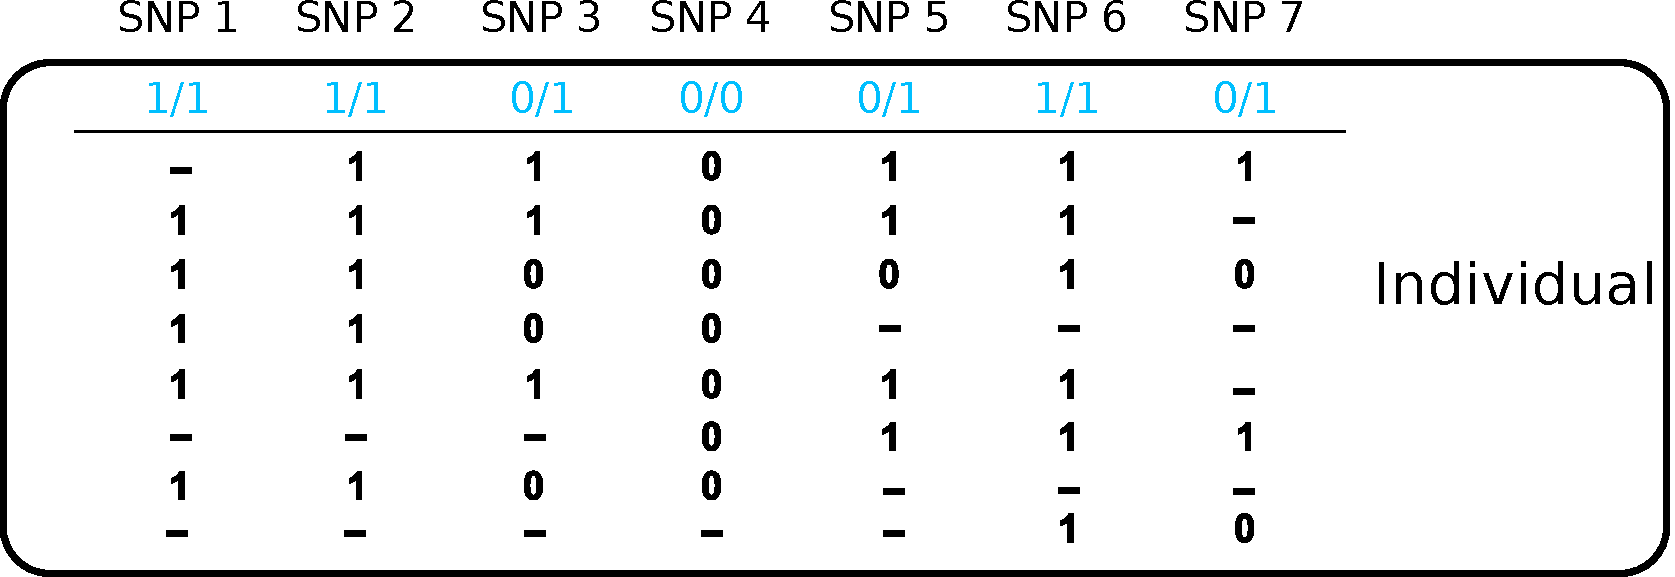
\includegraphics[scale=0.35]{figs/sih-phasing-complete-matrix.pdf}%
%width=0.85\textwidth
\end{center}
\end{frame}

\begin{frame}{Read-Based Phasing (Single Individual)}
	\begin{center}
\begin{block}{Input:}
		\begin{itemize}
		\color{blue}	\item $W \in \RR^{R \times M}$ : Matrix of confidence for each entry.

		\end{itemize}
	\end{block}
		\bigskip
		\bigskip
         \vspace*{1.9mm}
	\only<1>{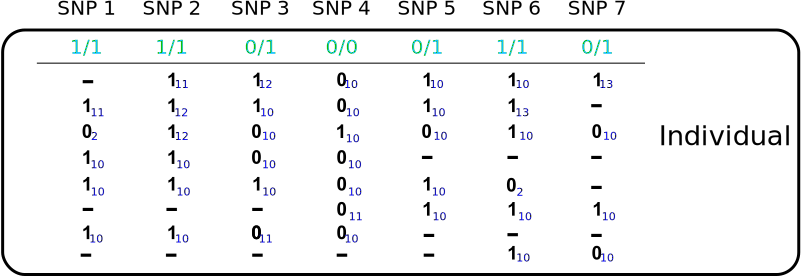
\includegraphics[scale=0.35]{figs/sih-phasing-complete-phred0}}
		\only<2>{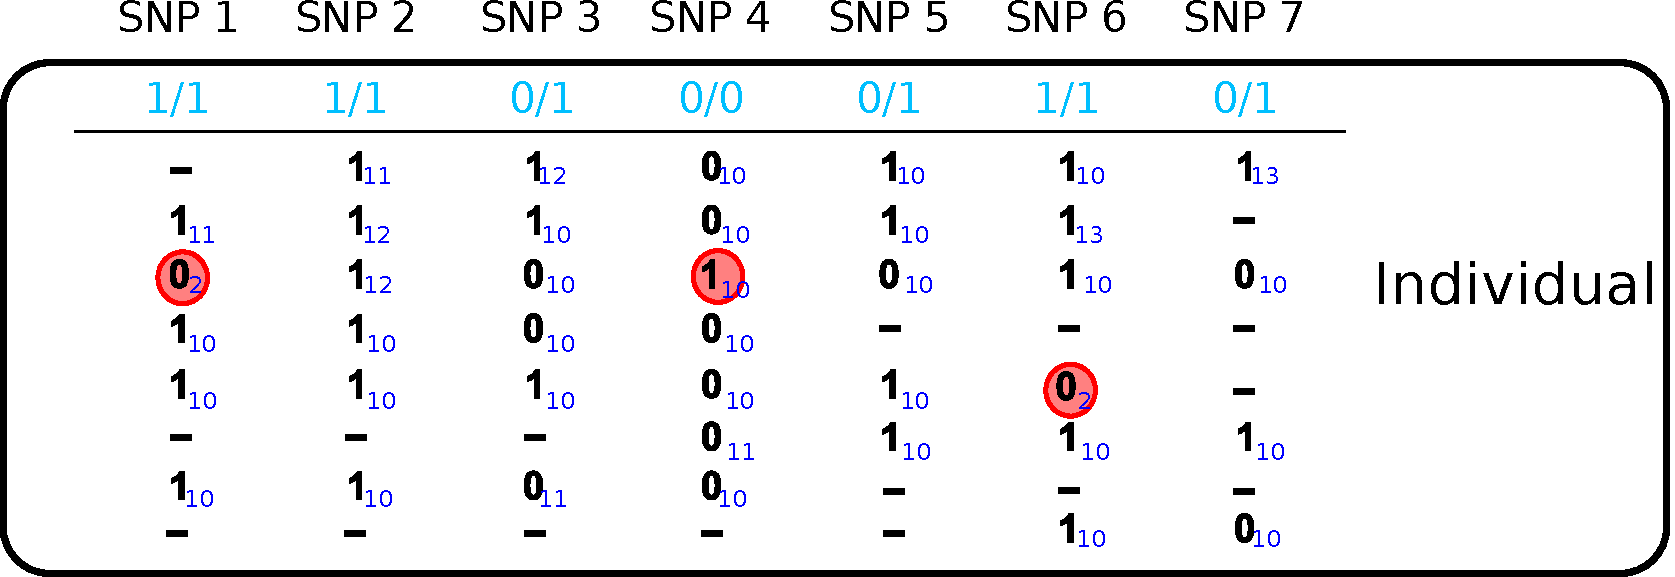
\includegraphics[scale=0.35]{figs/sih-phasing-complete-phred}}
%width=.9\textwidth
\end{center}
\end{frame}

\begin{frame}{Read-Based Phasing (Single Individual)}
	\vspace*{1.3mm}
	%\bigskip
	\begin{center}
		\begin{block}{Goal:}
			\begin{itemize}
				\item Conflict free matrix for an individual				
			\end{itemize}
		\end{block}
		\bigskip
		\bigskip
		\vspace*{2.23mm}
		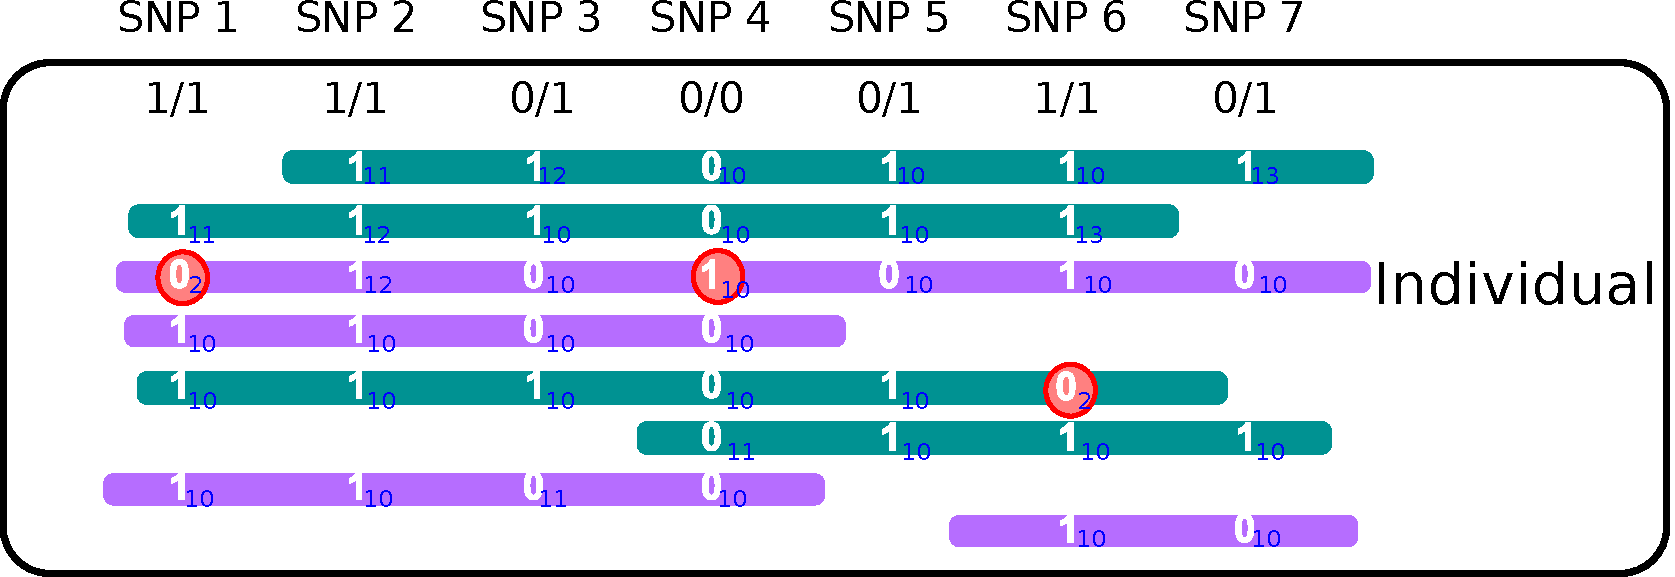
\includegraphics[scale=0.35]{figs/sih-phasing-complete4.pdf}
		%width=.9\textwidth
	\end{center}
\end{frame}

\begin{frame}{Read-Based Phasing (Single Individual)}
	%\vspace*{1.3mm}
	%\bigskip
	\begin{center}
	\begin{block}{Objective function: \color{red}wMEC }

		Flip the set of entries with minimum cost such that a conflict-free bipartition of rows exist.
		\begin{center}
			minimize $\sum_{(j,k)\in E}W(j,k)$
		\end{center}
		
	\end{block}
		\bigskip
		%\bigskip
		\vspace*{.6mm}
		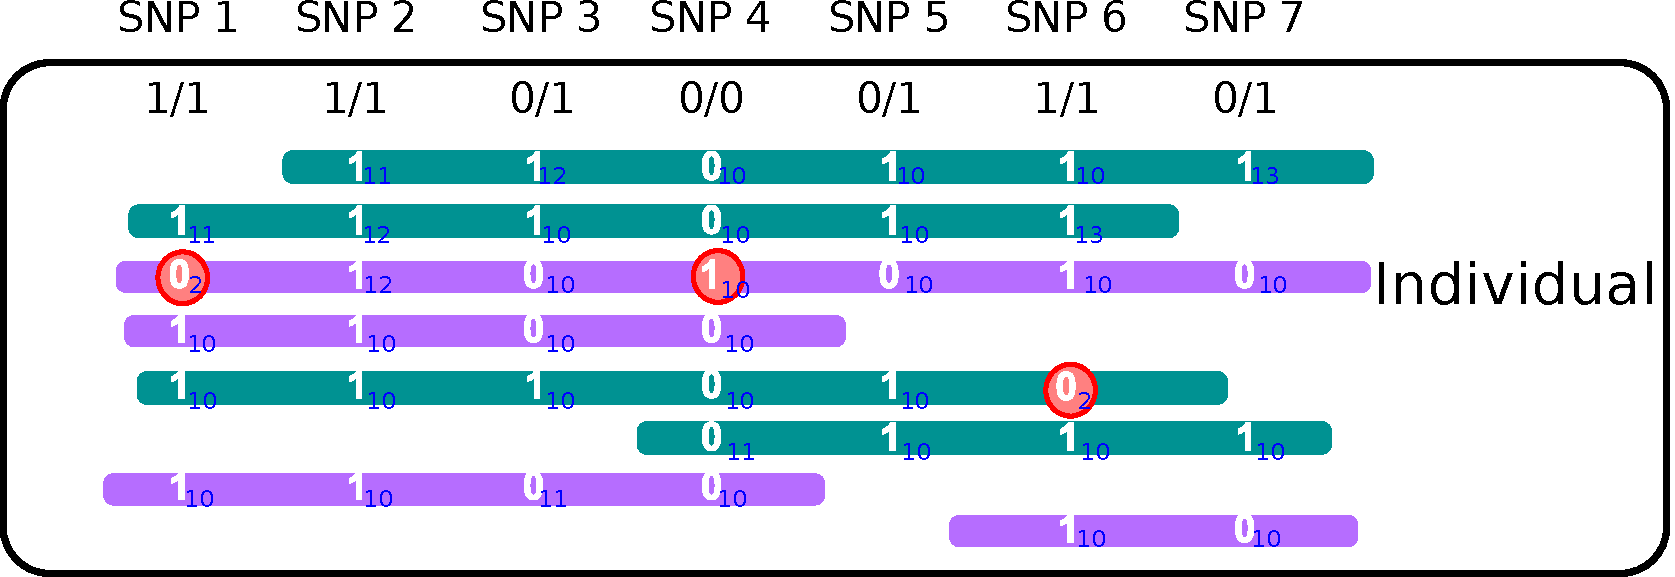
\includegraphics[scale=0.35]{figs/sih-phasing-complete4.pdf}\\
		\begin{center}
			
\includegraphics[width=.9\textwidth]{figs/sih-phasing-complete-haplo-goal1}
		\end{center}
			
		%width=.9\textwidth
	\end{center}
\end{frame}

%\begin{frame}{Read-Based Phasing (Single Individual)}
%\begin{center}
%\only<1->{
%	\begin{block}{Objective \color{red}wMEC }
%							Flip the entries with minimum cost such that a conflict-free bipartition of rows exist.
%		\begin{center}
%	minimize $\sum_{(j,k)\in E}\mathcal{W}(j,k)$
%		\end{center}
%		
%	\end{block}}	
%		%\visible<2>{
%
%				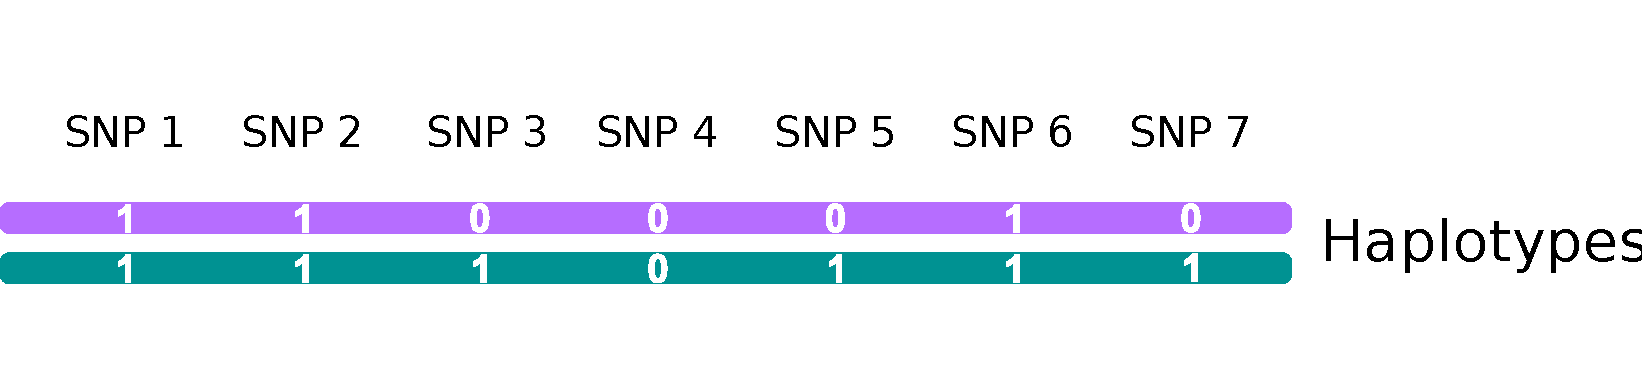
\includegraphics[width=.9\textwidth]{figs/sih-phasing-complete-haplo-goal}
%								\begin{block}{Goal:}
%									\begin{itemize}
%										\item $h^{0}, h^{1} \in \{0,1\}^{M}$: Haplotypes for an individual
%									\end{itemize}	
%								\end{block}
%	%}%
%\end{center}
%\end{frame}


\begin{frame}{WhatsHap Algorithm (Sketch)}
		\begin{block}{}
			Introduced at RECOMB 2014
		\end{block}
\begin{block}{}
\emph{Approach:} FPT algorithm with ``coverage'' as parameter.
\begin{itemize}
% \item \emph{coverage:} number of non-dash (i.e.~0,1) positions in a column
 \item Can be bounded without loosing relevant information
 \item Dynamic Programming
\end{itemize}
\end{block}
% \begin{center}
% 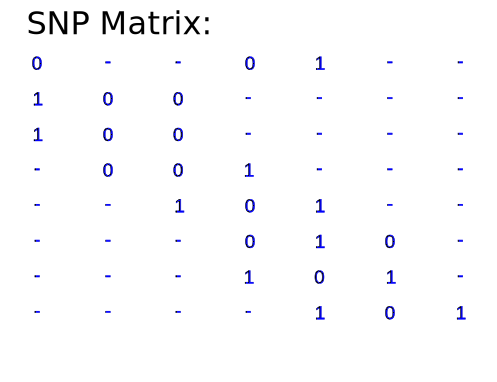
\includegraphics[width=0.5\textwidth]{figs/phasing-problem5}
% \end{center}
% \vspace{-2em}
%\begin{block}<2->{Dynamic Programming}
%Proceed \emph{column-wise}. For each column:
% \begin{enumerate}
%  \item \emph{Enumerate all bipartitions} of rows that cover that column
%  \item Compute number of bit-flips incurred by each bipartition
%  \item Project costs to ``intersection column''
% \end{enumerate}
%\end{block}
\end{frame}

%\begin{frame}{Runtime}
%\begin{block}{Notation}
%\begin{itemize}
% \item \emph{$c$: maximum coverage}, i.e.\ maximum number of active reads per column
% \item \emph{$M$: number of columns}, i.e.\ number of variants to be phased
%\end{itemize}
%\end{block}
%\begin{block}{Runtime}
%\[O(2^c\cdot M)\]
%\end{block}
%\begin{block}{Conclusions}
%\begin{itemize}
% \item Linear in the number of variants (good)
% \item Independent of read length (good, especially for long reads)
% \item Exponential in the coverage (no big problem in practice, can prune to, say, 15$\times$)
%\end{itemize}
%\end{block}
%\end{frame}

\captionslide{Read-Based Phasing of\\ Related Individuals\\
{ \begin{enumerate} \scriptsize \color{red}
		\item How much coverage is needed for resolving haplotypes in related individuals as opposed to single individual?
		\item Can we get long-range haplotypes for all the individuals?
	\end{itemize} }
}

\begin{frame}{Phasing Related Individuals}

\begin{center}
	\only<1>{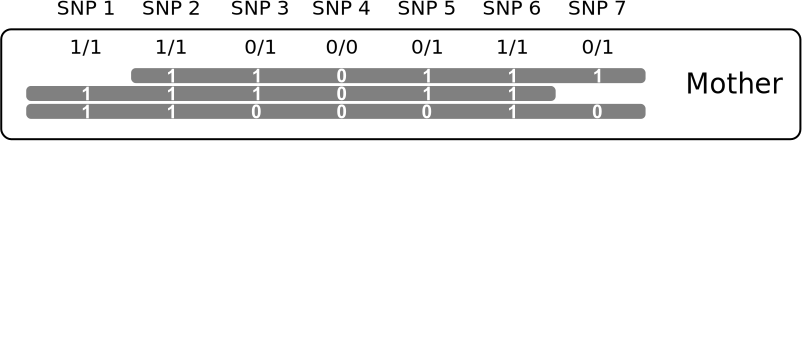
\includegraphics[width=.9\textwidth]{figs/trio-phasing-complete1}\vspace*{2.05cm}}%
	\only<2>{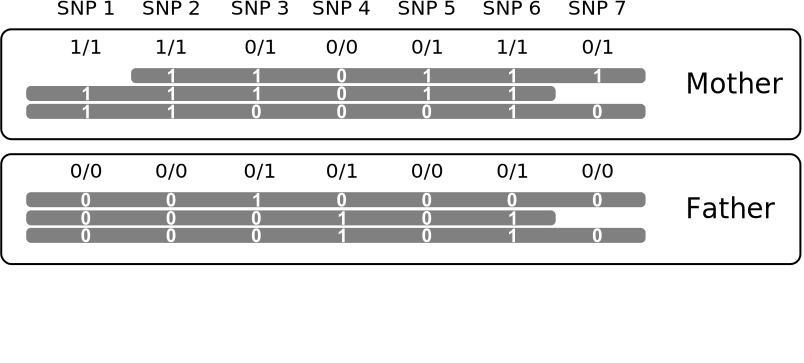
\includegraphics[width=.9\textwidth]{figs/trio-phasing-complete2}\vspace*{2.05cm}}%
	\only<3>{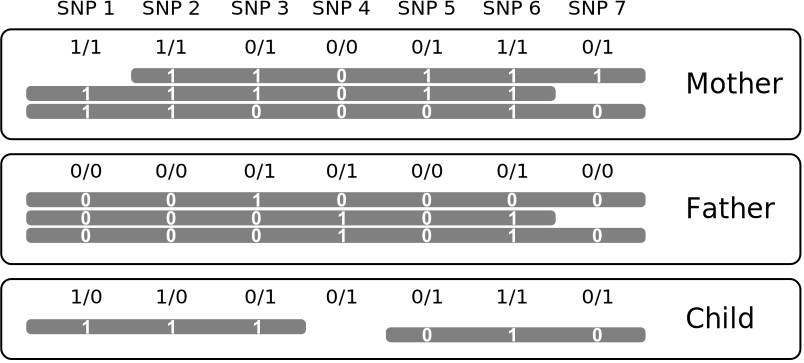
\includegraphics[width=.9\textwidth]{figs/trio-phasing-complete3}
		\begin{block}{}
			\begin{itemize}
				\item \emph{Genetic haplotyping:} cannot phase SNP 3 (all heterozygous)
				\item \emph{Read-based haplotyping:} cannot connect SNP 4 in child
				\item Solution: \emph{combine genetic and read-based haplotyping}
			\end{itemize}
		\end{block}}%
%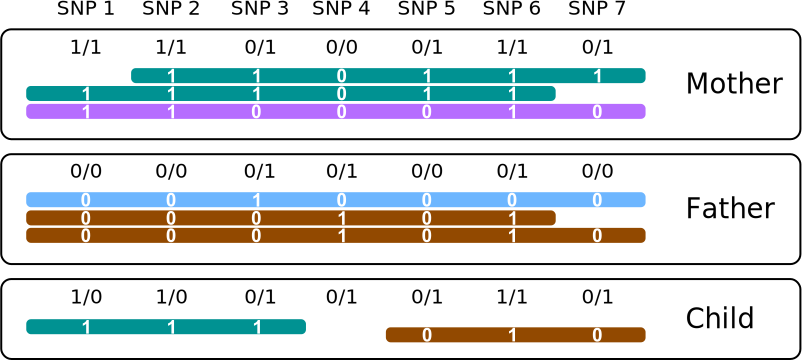
\includegraphics[width=.9\textwidth]{figs/trio-phasing-complete}
\end{center}
\end{frame}

\begin{frame}{Phasing Related Individuals}
	\begin{center} \vspace*{.5mm}
		\only<1>{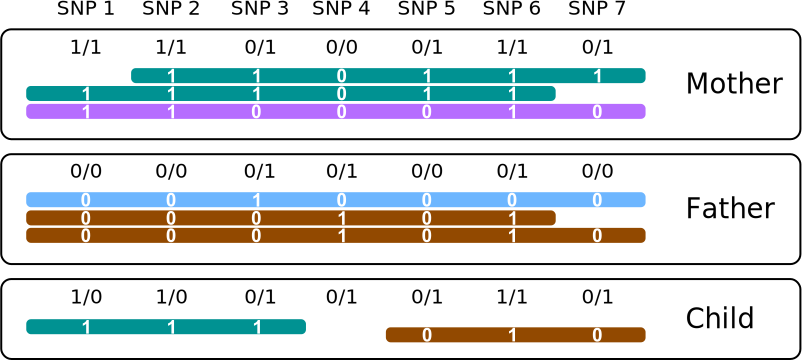
\includegraphics[width=.9\textwidth]{figs/trio-phasing-complete}}%
		%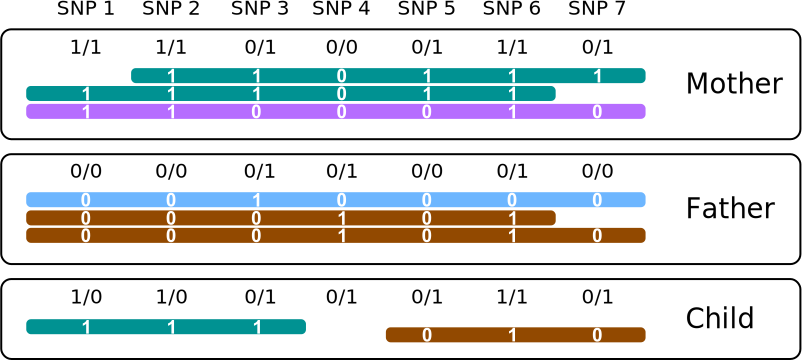
\includegraphics[width=.9\textwidth]{figs/trio-phasing-complete}

		\begin{block}{}
			\begin{itemize}
				\item \emph{Genetic haplotyping:} cannot phase SNP 3 (all heterozygous)
				\item \emph{Read-based haplotyping:} cannot connect SNP 4 in child
				\item Solution: \emph{combine genetic and read-based haplotyping}
			\end{itemize}
		\end{block}
			\end{center}
					\vspace*{4.5mm}
\end{frame}


%\begin{frame}{Phasing Related Individuals}
%\begin{block}{Input:}
%\begin{itemize}
% %\item $\I$ : Set of individuals, $\T$ : Set of trio relationships
%  \item $g_i \in \{0,1,2\}^M$ : Input genotype for individual $i$
%			 \item $\F_i \in \{0,1,-\}^{R_i\times M}$ : Input SNP matrix for individual $i$ 
%
% \end{itemize}
%\end{block}
%\begin{center}
%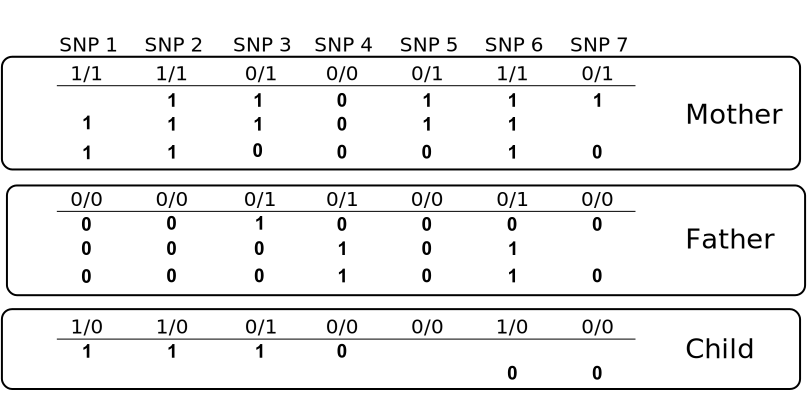
\includegraphics[width=.9\textwidth]{figs/trio-phasing-complete-matrix}
%\end{center}
%\end{frame}
%
%
%
%\begin{frame}{Phasing Related Individuals}
%	\begin{block}{Input:}
%		\begin{itemize}
%
%			\item $\W_i \in \RR^{R_i \times M}$ : Matrix of phred scores for individual $i$
%			%\item $\A(k)$ : Set of reads active in column $k$
%		\end{itemize}
%	\end{block}
%	\vspace*{5.5mm}
%	\begin{center}
%		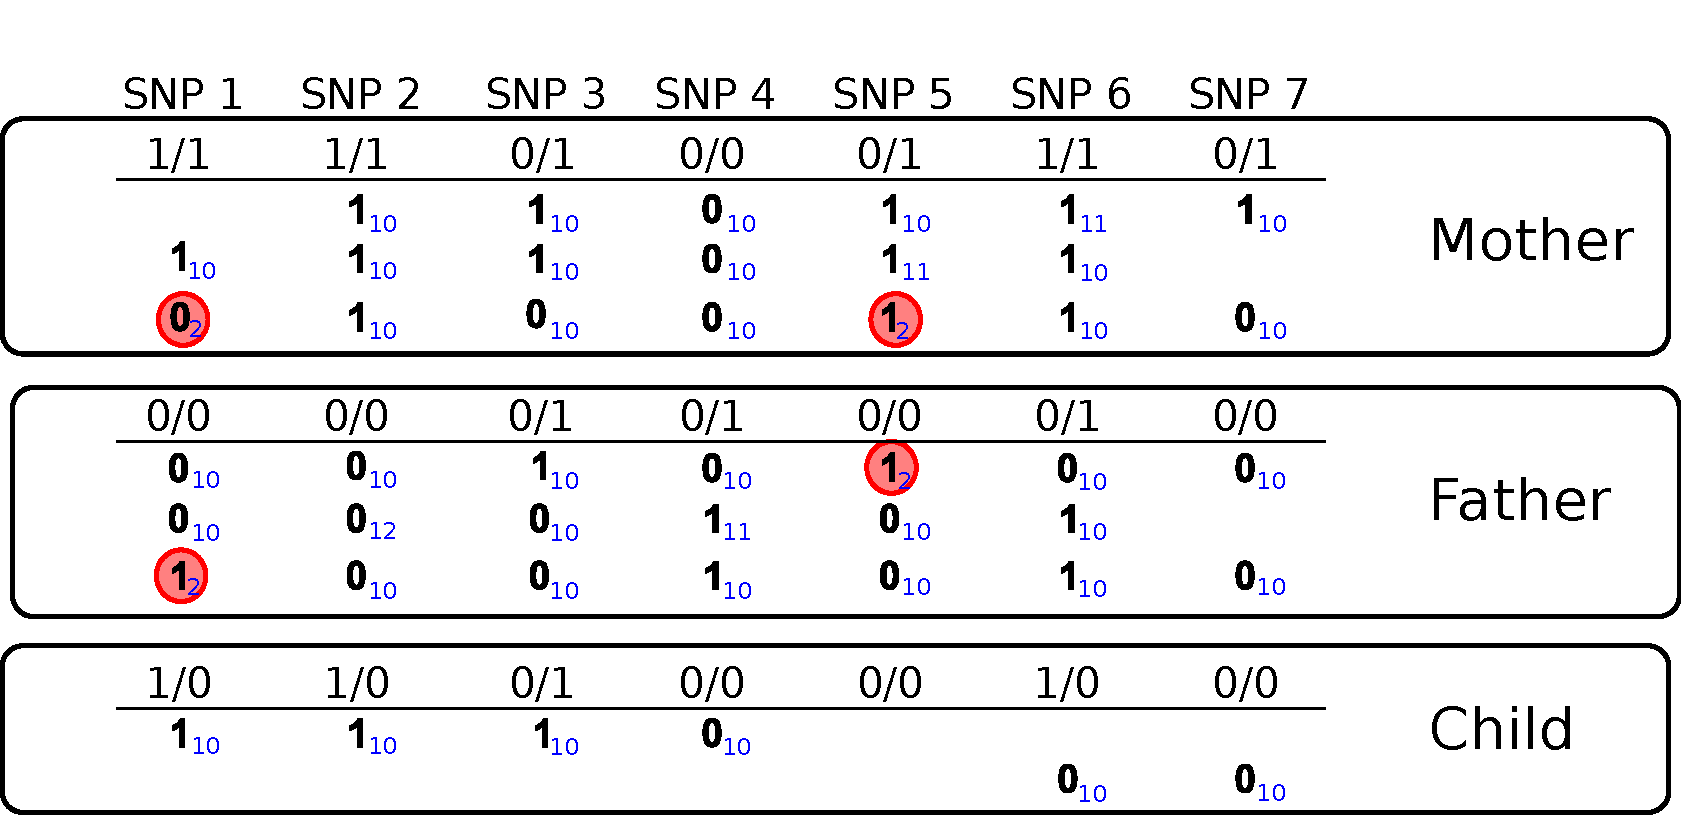
\includegraphics[width=.9\textwidth]{figs/trio-phasing-complete-phred}
%	\end{center}
%\end{frame}
%
%\begin{frame}{Phasing Related Individuals}
%	\begin{block}{Input:}
%		\begin{itemize}
%			\item $\X \in \RR^M$ : Recombination cost vector
%			\item $t_{m\rightarrow c}, t_{f\rightarrow c} \in \{0,1\}^M$ : transmission vectors for trio
%		\end{itemize}
%	\end{block}
%	\begin{center}
%		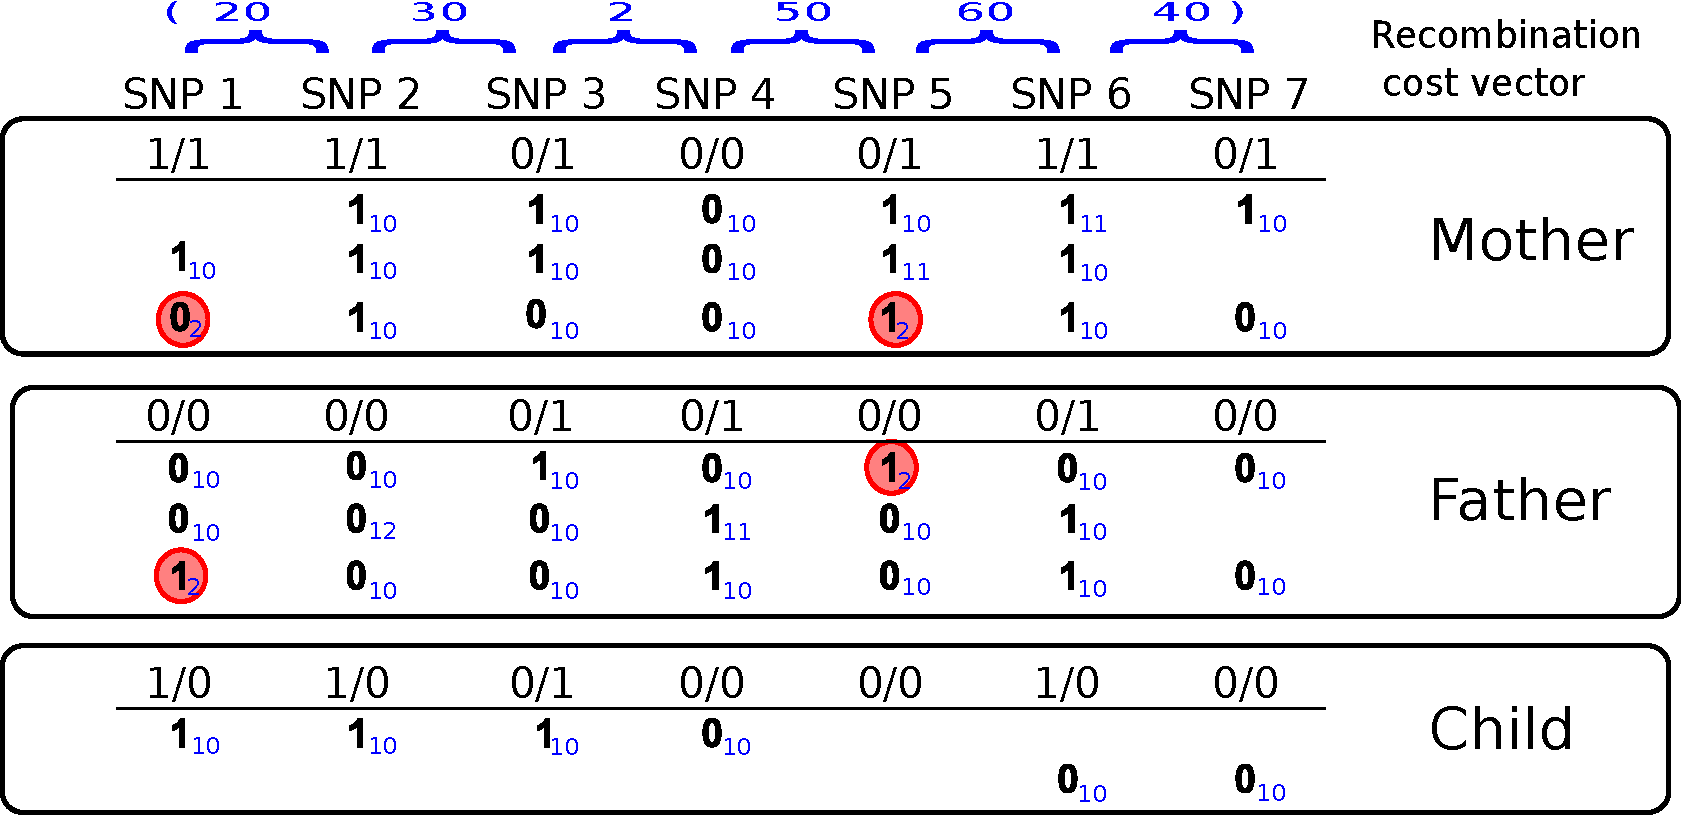
\includegraphics[width=.9\textwidth]{figs/trio-phasing-complete-recomb-vector}
%	\end{center}
%\end{frame}

%\begin{frame}{Phasing Related Individuals}
%	\begin{block}{Goal:}
%		\begin{itemize}
%			\item Conflict free matrix by following Mendelian Inheritance.
%			\item Meiotic Recombination
%		\end{itemize}
%	\end{block}
%	\vspace*{1.4mm}
%	\begin{center}
%		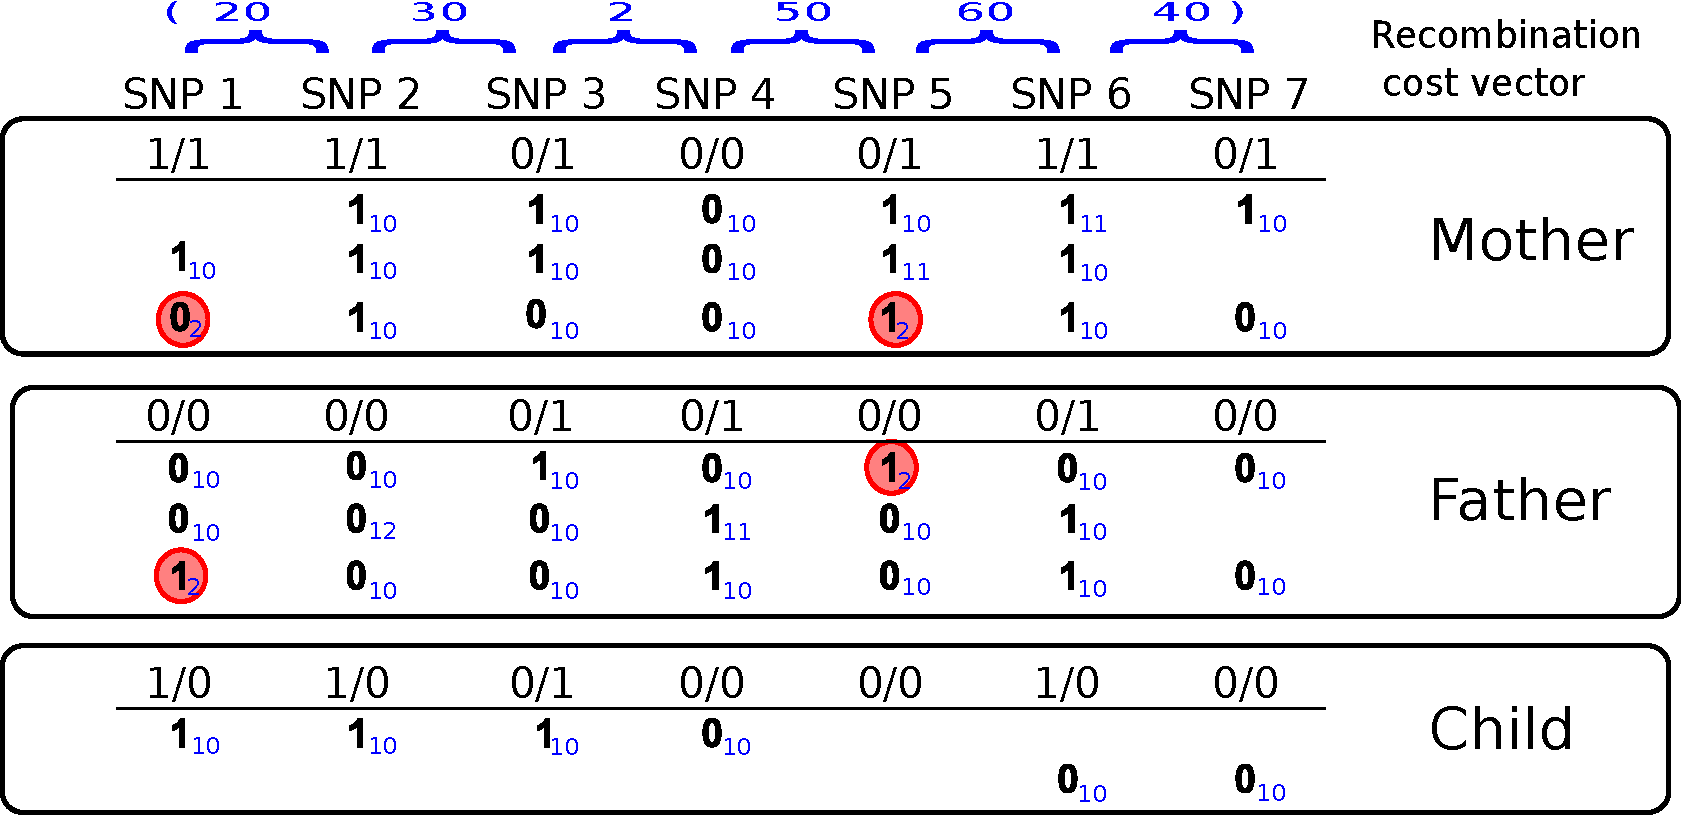
\includegraphics[width=.9\textwidth]{figs/trio-phasing-complete-recomb-vector}
%	\end{center}
%\end{frame}

%\begin{frame}{Phasing Related Individuals}
%	\begin{block}{}
%		\begin{itemize}
%			\item \emph{Genetic haplotyping:} cannot phase SNP 3 (all heterozygous)
%			\item \emph{Read-based haplotyping:} cannot connect SNPs 3-5 in child
%			\item Solution: \emph{combine genetic and read-based haplotyping}
%		\end{itemize}
%	\end{block}
%	\begin{center}
%		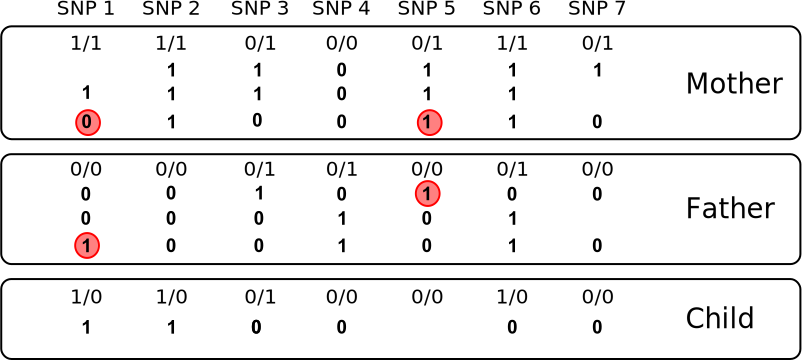
\includegraphics[width=.9\textwidth]{figs/trio-phasing-complete-error}
%	\end{center}
%\end{frame}

\begin{frame}{From wMEC to ``MEC on Pedigrees'' (PedMEC)}
	\begin{center}
		\only<1>{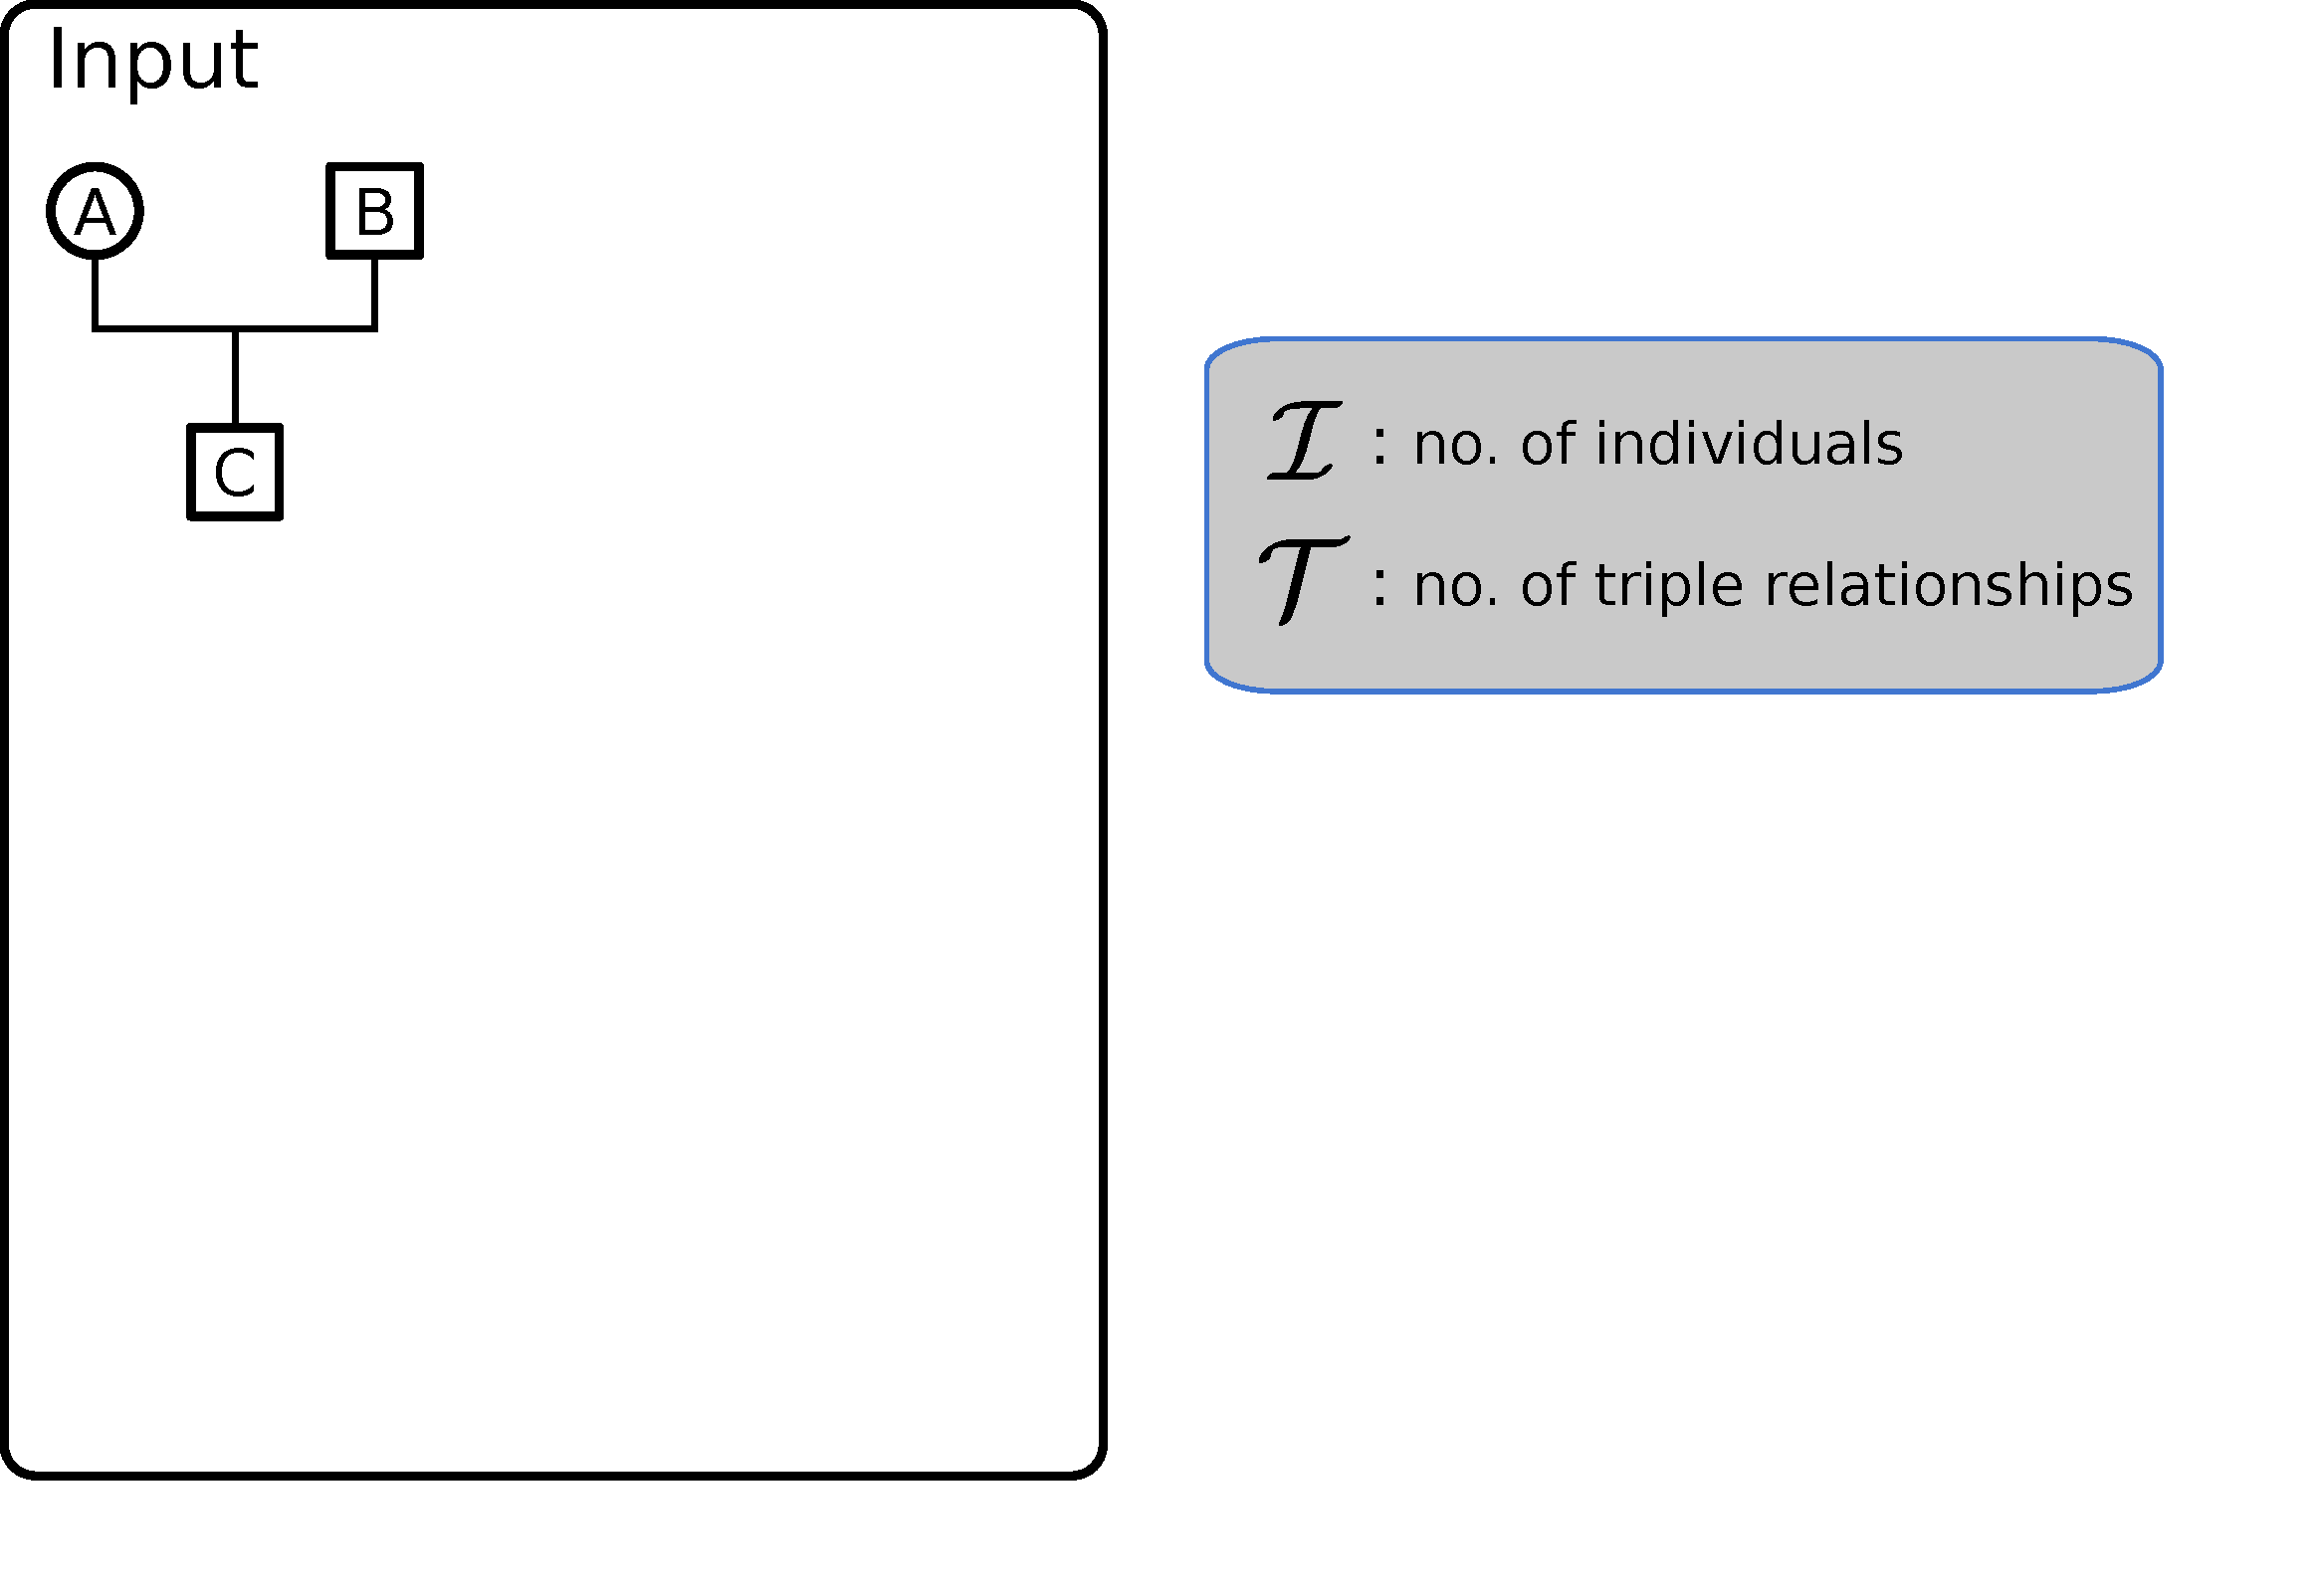
\includegraphics[width=\textwidth, height=175]{figs/pedmec1}}%
		\only<2>{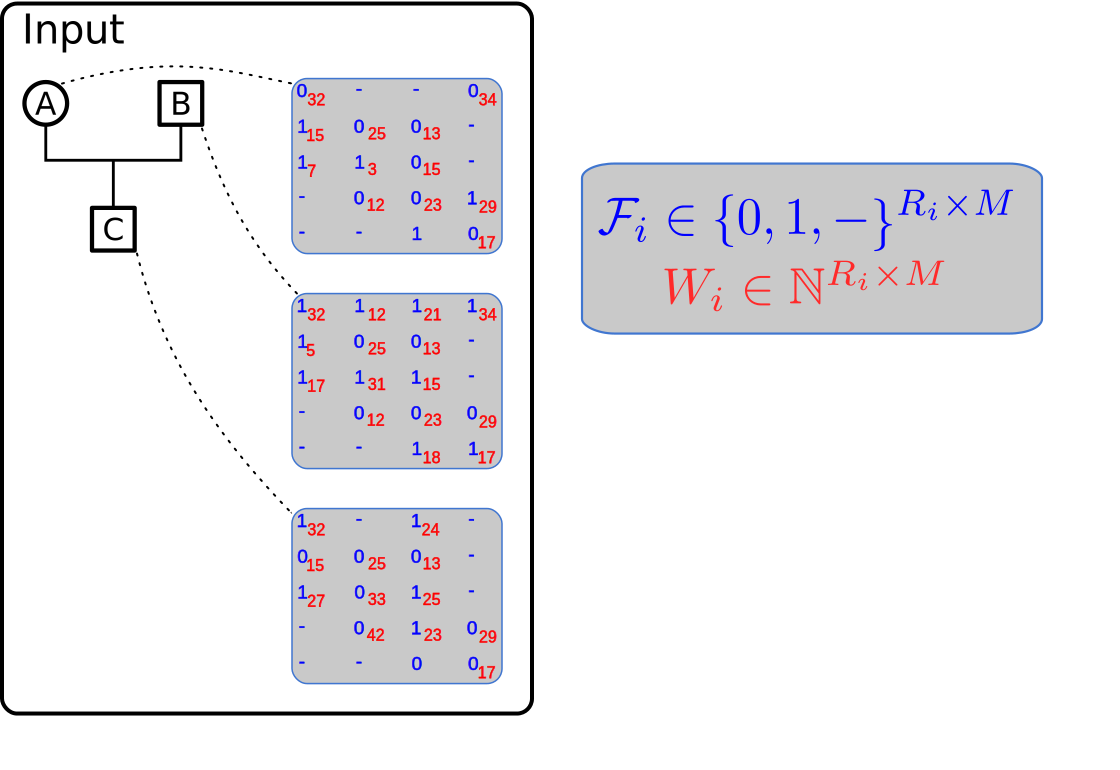
\includegraphics[width=\textwidth, height=175]{figs/pedmec2}}%
		\only<3>{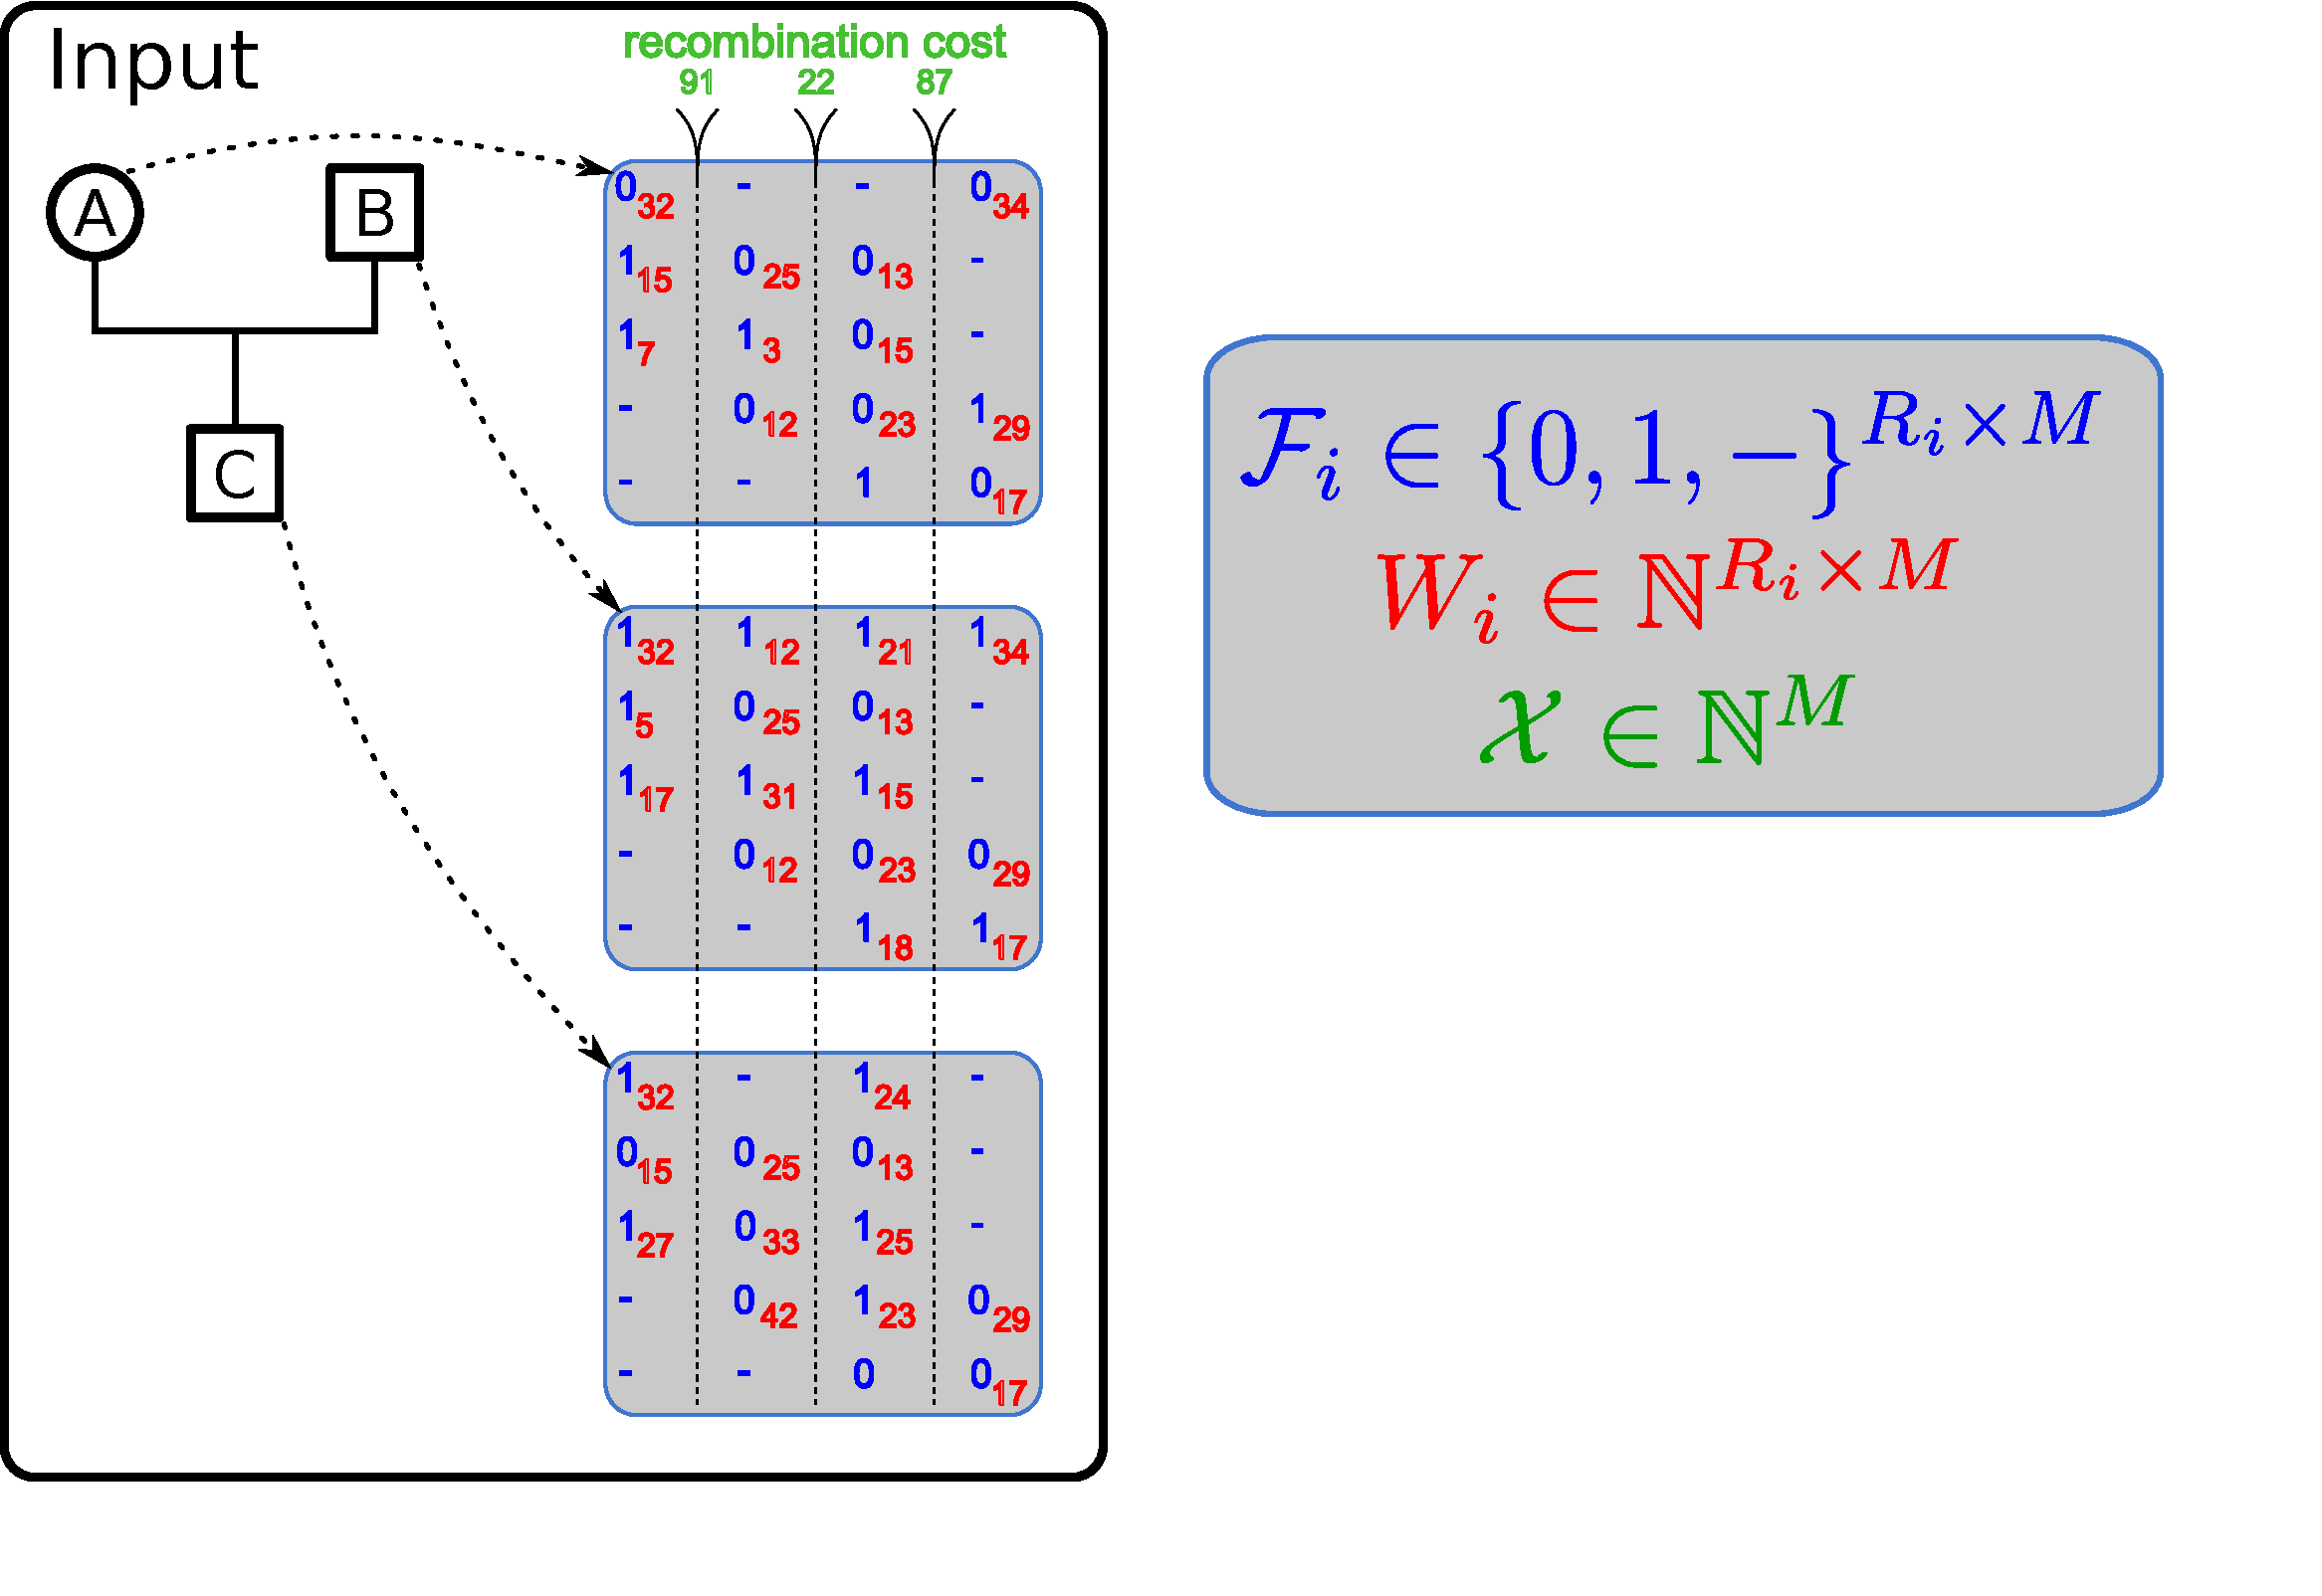
\includegraphics[width=\textwidth, height=175]{figs/pedmec3}}%
		\only<4>{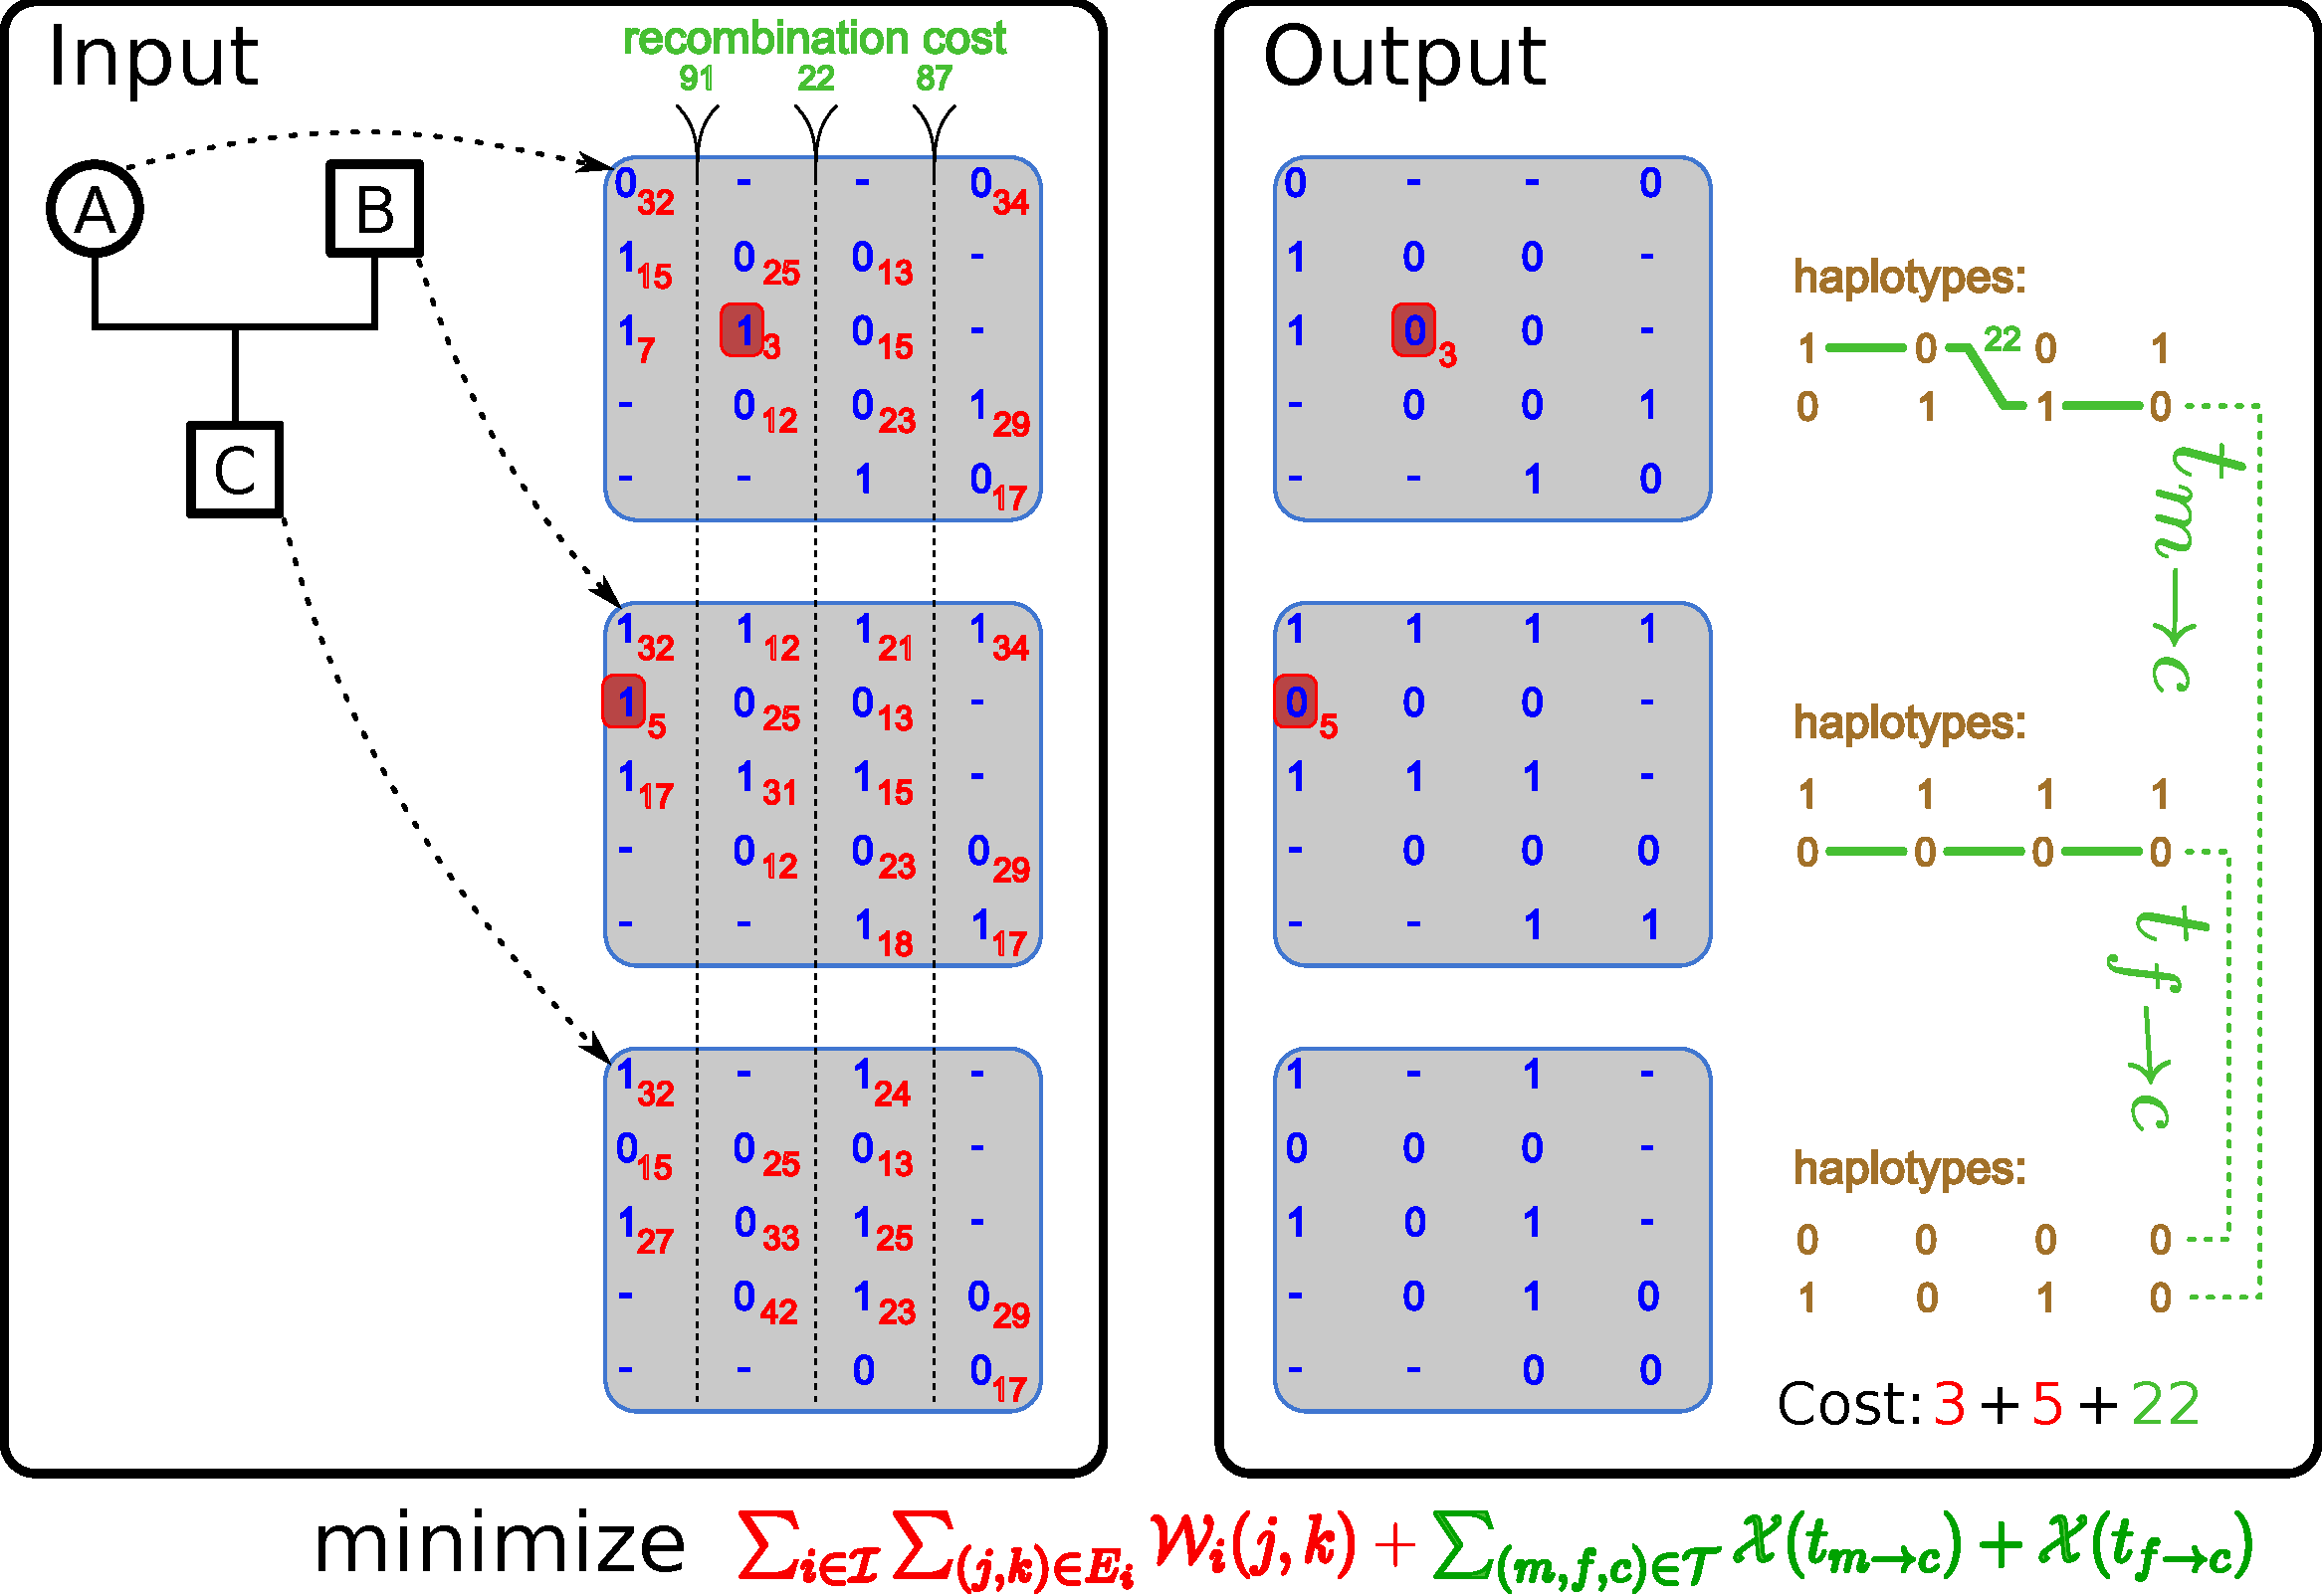
\includegraphics[width=\textwidth, height=175]{figs/pedmec4}}%
			%	\only<5>{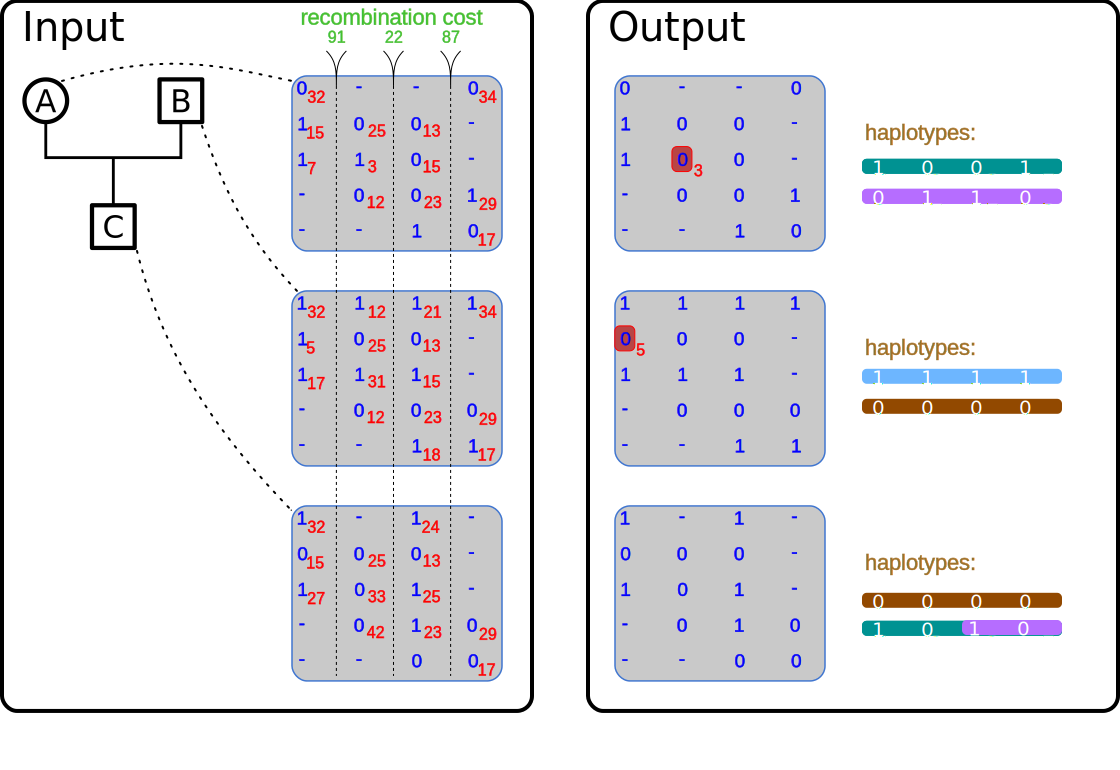
\includegraphics[width=\textwidth, height=175]{figs/pedmec5}}%
	\end{center}
\end{frame}

%\begin{frame}{From wMEC to ``MEC on Pedigrees'' (PedMEC)}
%			\begin{block}{Objective function (minimize):\color{red}PedMEC }
%				\scriptsize
%				\begin{itemize}
					%\item[] \[\sum_{i\in\mathcal{I}}\sum_{(j,k)\in E_i}\mathcal{W}_i(j,k)+\sum_{(m,f,c)\in\mathcal{T}}\mathcal{X}(t_{m\to c}) + \mathcal{X}(t_{f\to c})\] 
				%\end{itemize}
		%		
		%	\end{block}

		%	\visible<2->{\begin{center}
		%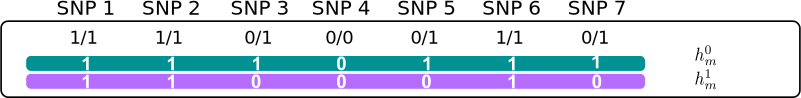
\includegraphics[width=.9\textwidth]{figs/trio-phasing-complete-haplotype3}
	%\end{center}}
	%			\visible<3->{\begin{center}
	%					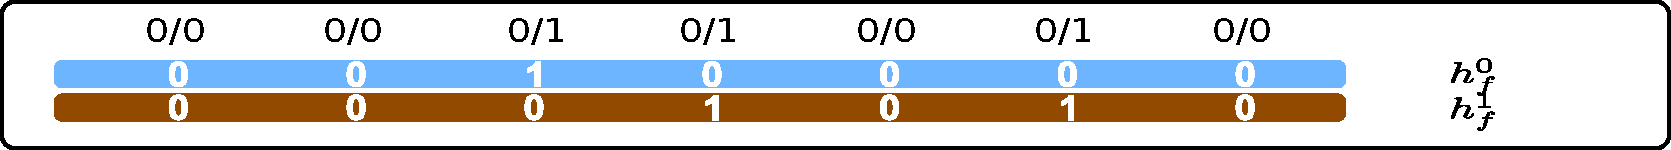
\includegraphics[width=.9\textwidth]{figs/trio-phasing-complete-haplotype2}
	%				\end{center}}
	%							\visible<4->{\begin{center}
	%									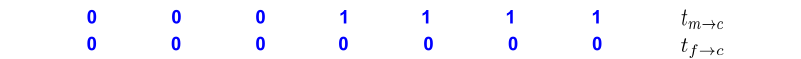
\includegraphics[width=.9\textwidth]{figs/trio-phasing-complete-haplotype1}
	%								\end{center}}
	%											\begin{center}
	%													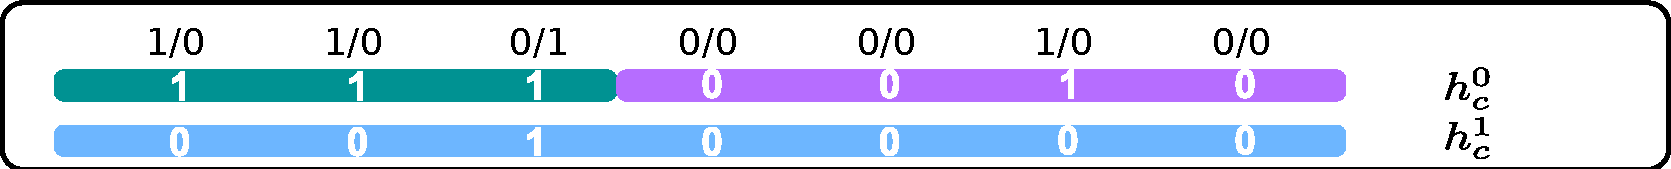
\includegraphics[width=.9\textwidth]{figs/trio-phasing-complete-haplotype}
	%												\end{center}
	%												\begin{block}{Goal:}
	%													\begin{center}
	%														\scriptsize  $h^{0}_{i}, h^{1}_{i} \in \{0,1\}^{M}$: Haplotypes for individual $i$
	%													\end{center}	
	%												\end{block}
		%\visible<6->{\begin{block}{Goal:}
		%	\begin{center}
		%		\scriptsize  $h^{0}_{i}, h^{1}_{i} \in \{0,1\}^{M}$: Haplotypes for individual $i$
		%	\end{center}	
		%\end{block}}
%\end{frame}

\begin{frame}

		\begin{block}{WhatsHap (Related Individuals): \color{red} FPT }
			\begin{itemize}
				\item Use similar approach as for wMEC
				\item Add additional dimension to DP table: \emph{transmission status}\\
				i.e.\ which haplotype in each parent is transmitted to child
			\end{itemize}
		\end{block}
\end{frame}

\begin{frame}{WhatsHap (Related Individuals)}
	\begin{center}
		\only<1>{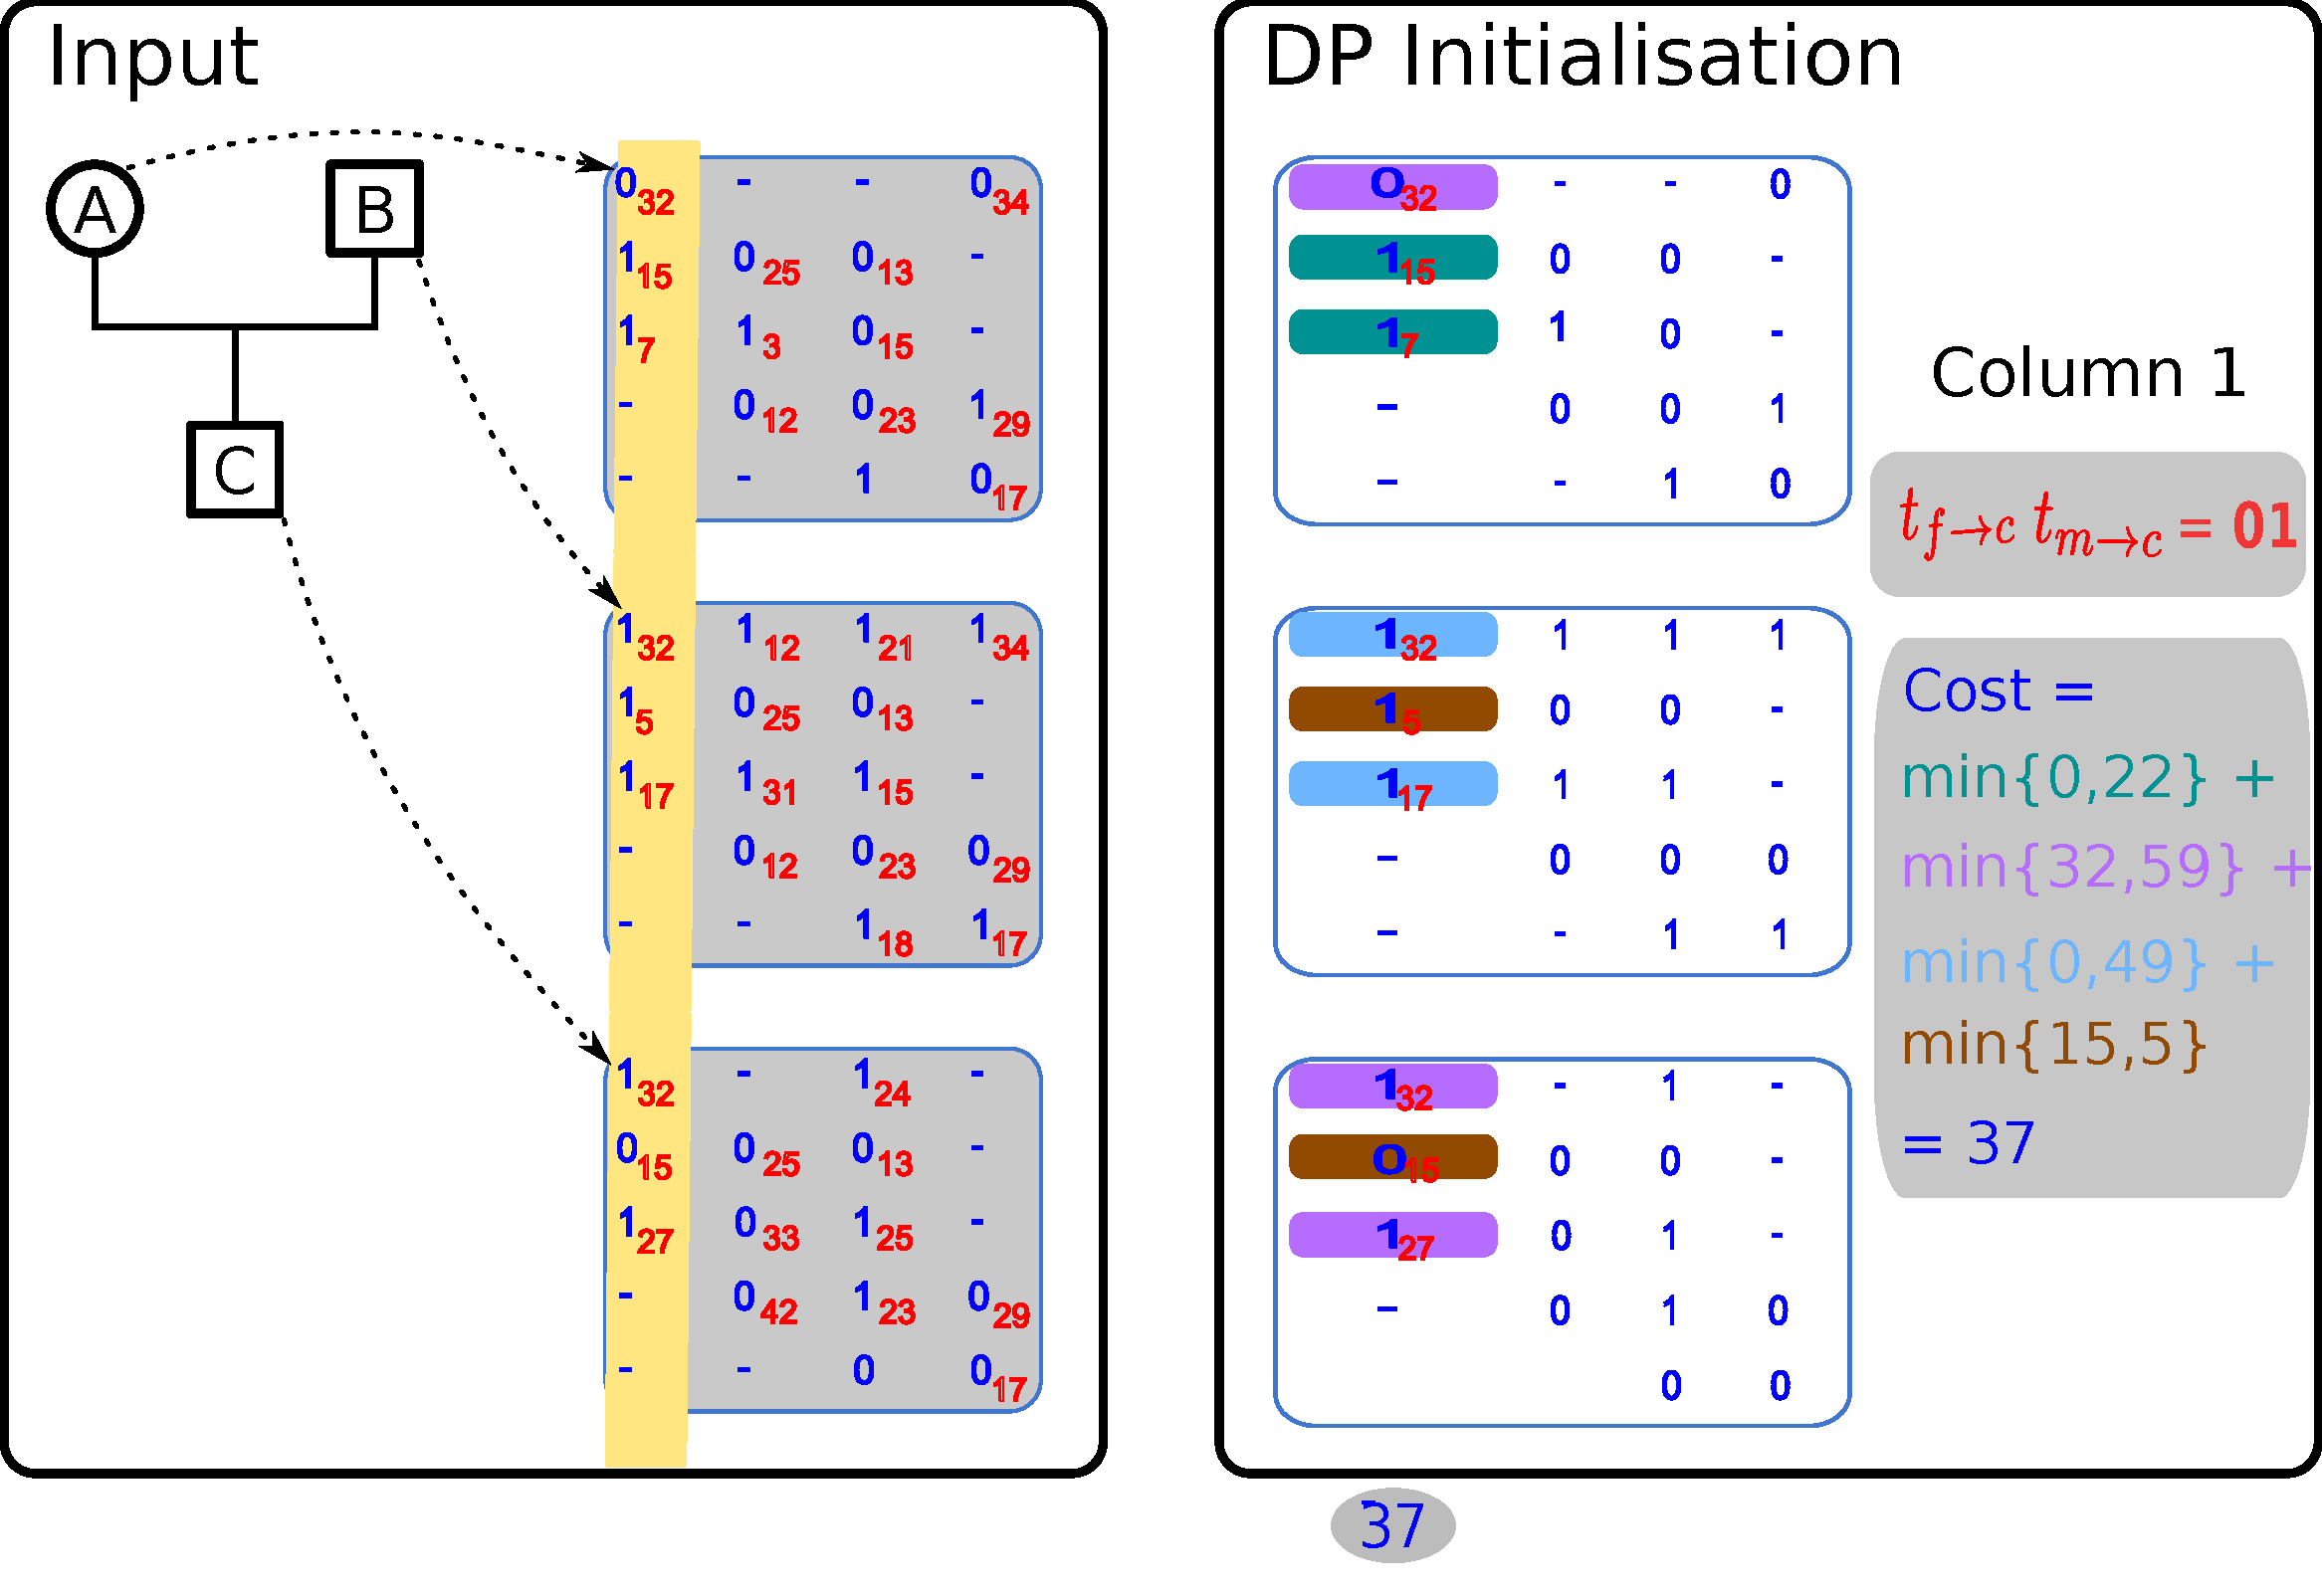
\includegraphics[width=\textwidth, height=175]{figs/pedmeccost2}}%
		\only<2>{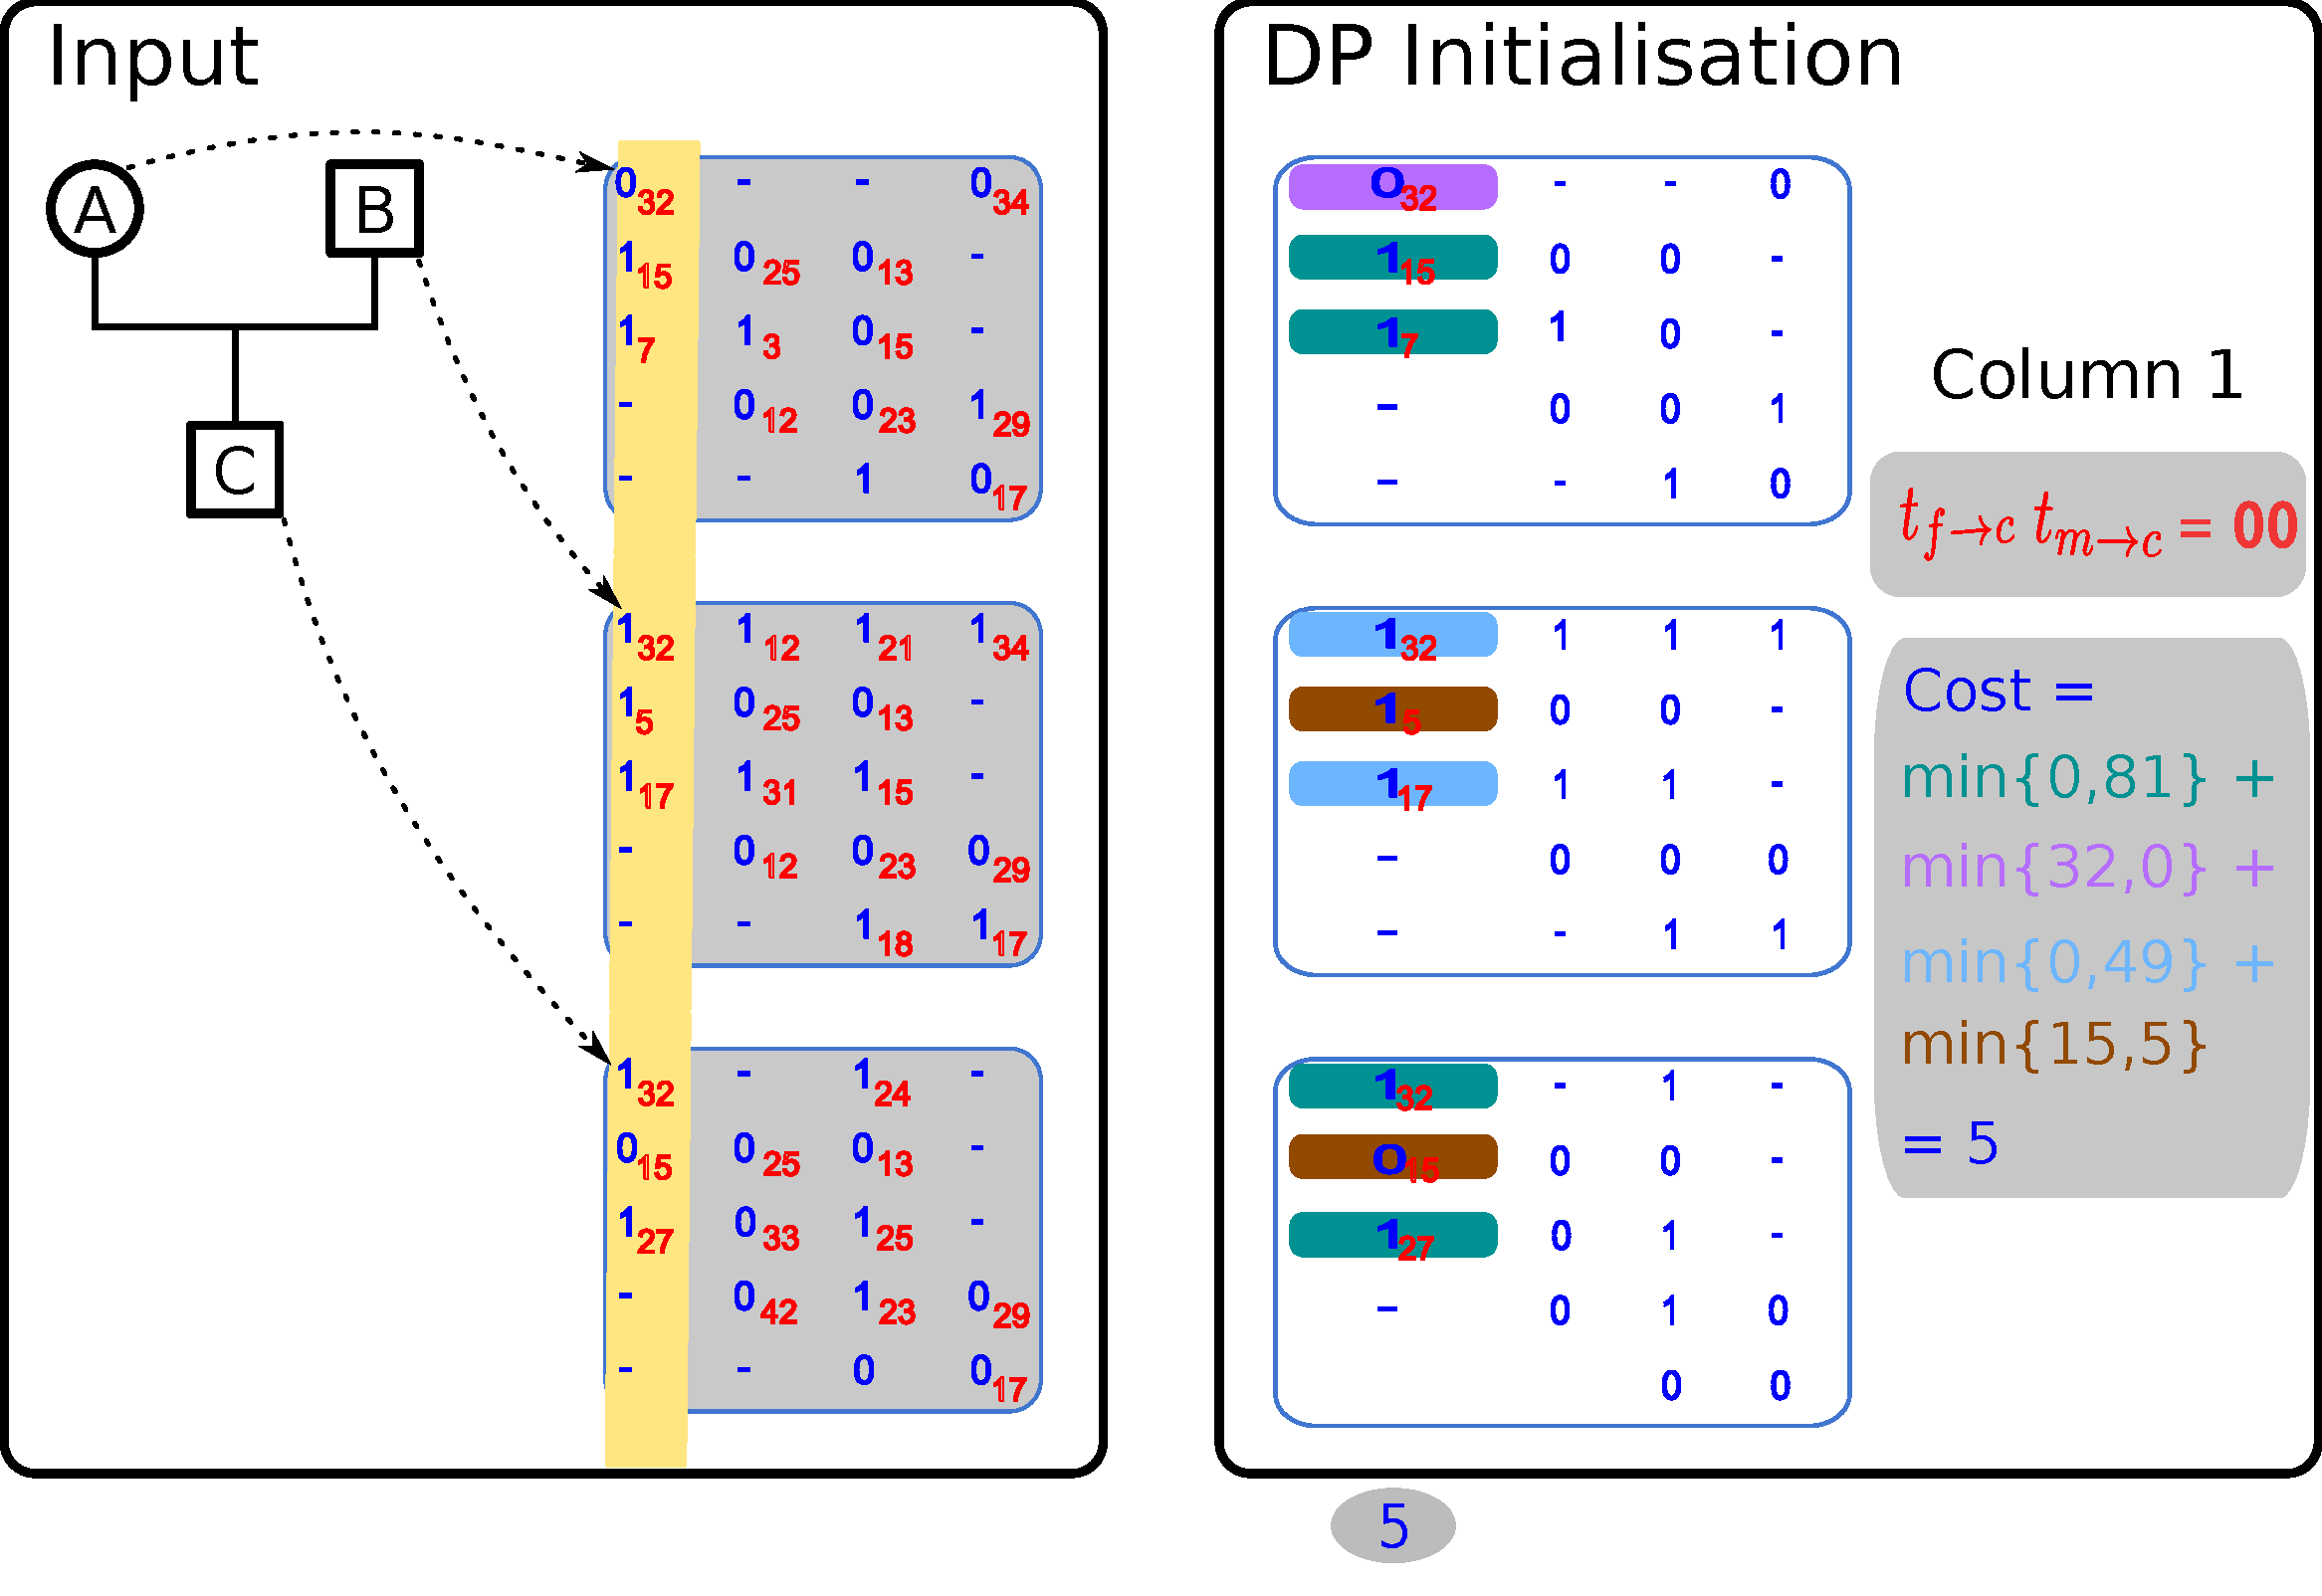
\includegraphics[width=\textwidth, height=175]{figs/pedmeccost1}}%
		\only<3>{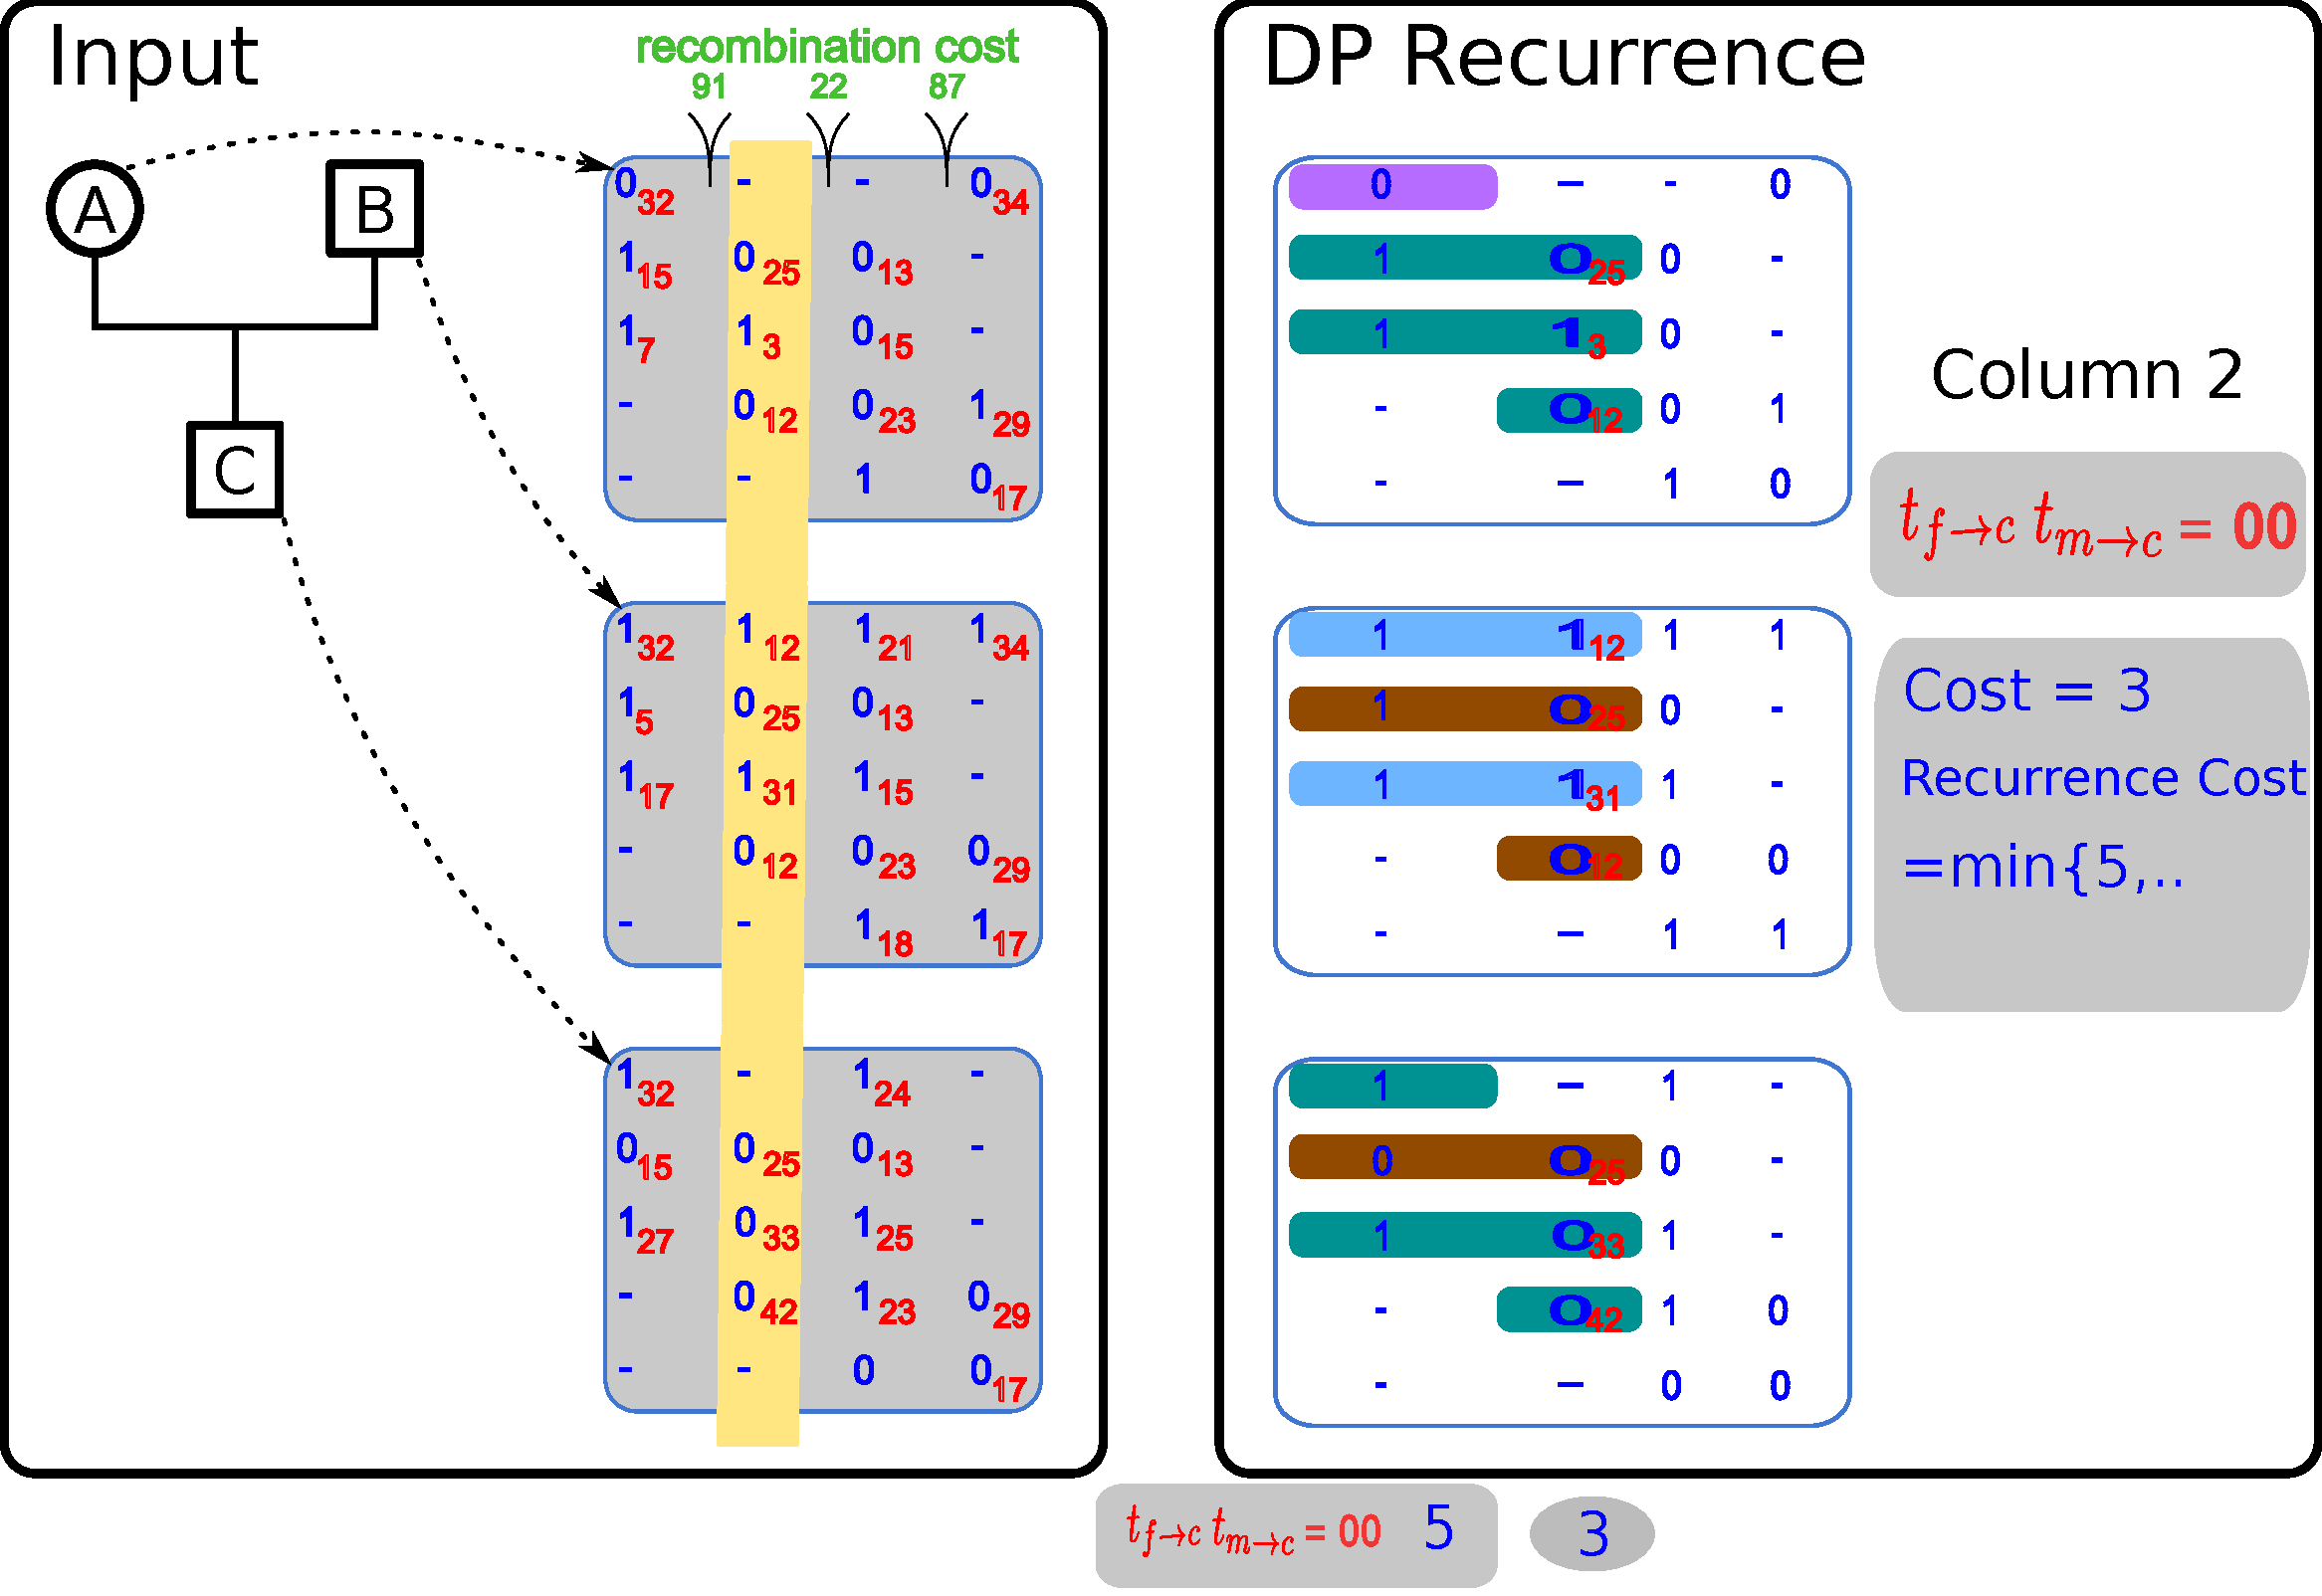
\includegraphics[width=\textwidth, height=175]{figs/pedmeccost3}}%
		\only<4>{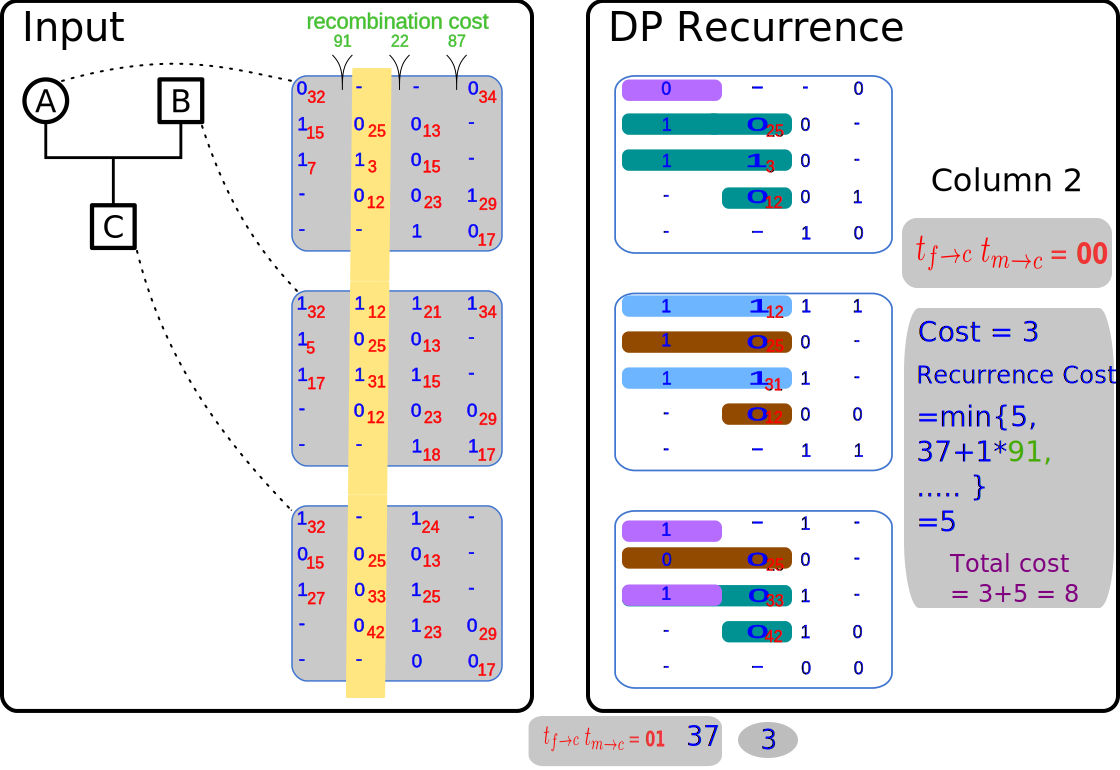
\includegraphics[width=\textwidth, height=175]{figs/pedmeccost4}}%
%		\only<5>{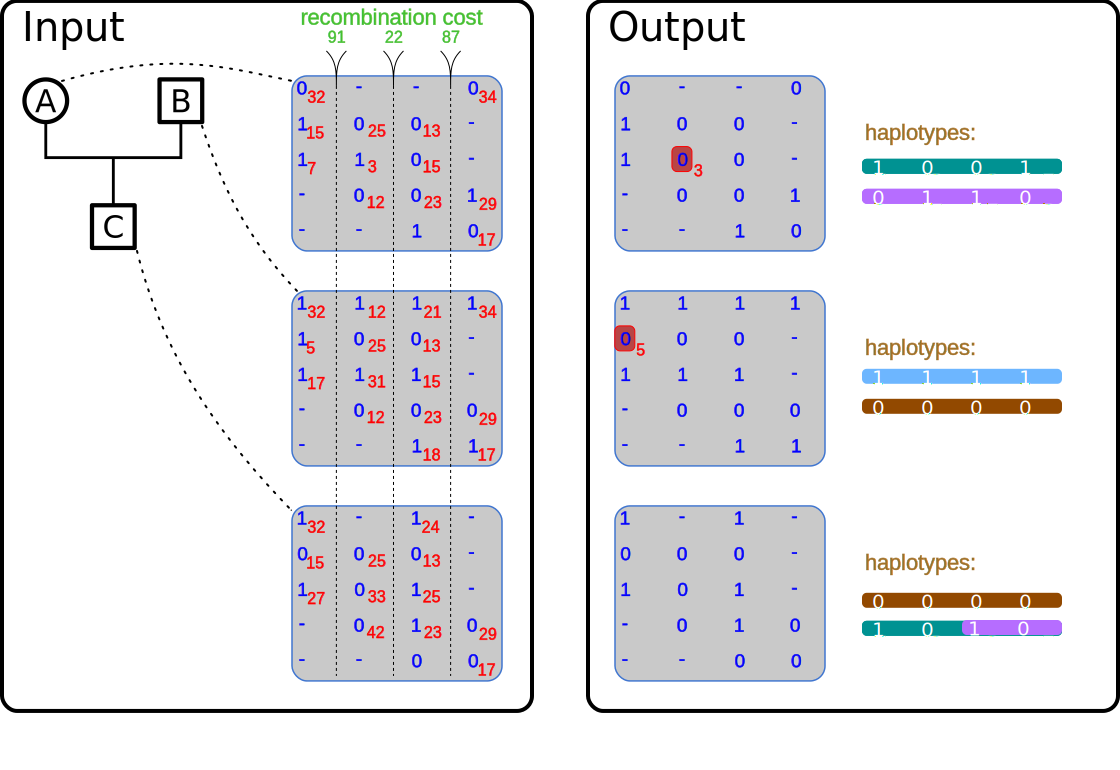
\includegraphics[width=\textwidth, height=180]{figs/pedmec5}}%
	\end{center}
\end{frame}

%\begin{frame}{WhatsHap (Related Individuals) }
%%	\begin{block}{WhatsHap (Related Individuals) }
%%                \scriptsize
%%		\textcolor{red}{DP Initialization}
%%		\begin{equation}\label{eqn:delta_c}
%%		\Delta_C(k,B,t)= \min_{a\in \{0,1\}^{\mathcal{S}(k,B,t)}}\left\{\sum_{S\in\mathcal{S}(k,B,t)}W_{k,S}^{a(S)}\right\},
%%		\end{equation}
%%	\end{block}
%%        \vspace*{6mm}
%
%		\begin{columns}[]
%			 \hspace*{10mm}
%			\begin{column}{0.4\textwidth}
%				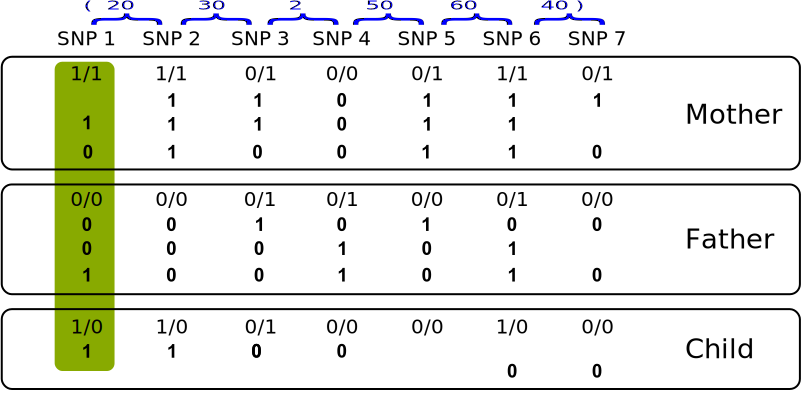
\includegraphics[scale=0.15]{figs/trio-phasing-complete-first-column}
%                                % width=0.9\textwidth
%                                \vskip5mm
%                                \vspace*{3mm}
%			\end{column}
%		\only<1>{                         \hspace*{1mm}
%				\begin{column}{0.9\textwidth}
%					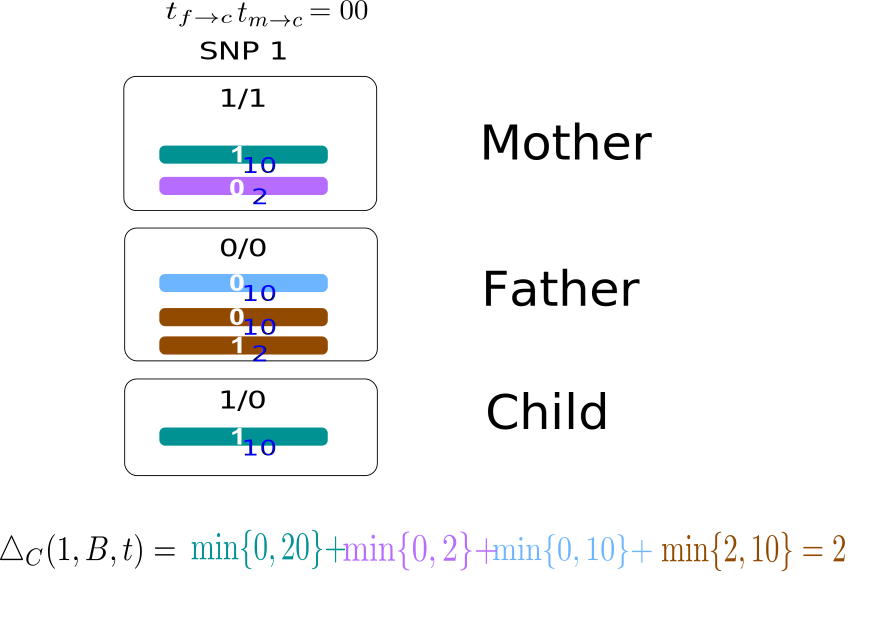
\includegraphics[height=.5\textwidth]{figs/trio-phasing-complete-cost-computation1-first-bipartition}
%                   \vskip5mm           
%			\end{column} 
%			\vskip5mm}
%			\only<2>{	     \hspace*{.2mm}
%						\begin{column}{0.9\textwidth}
%							%\begin{center}
%							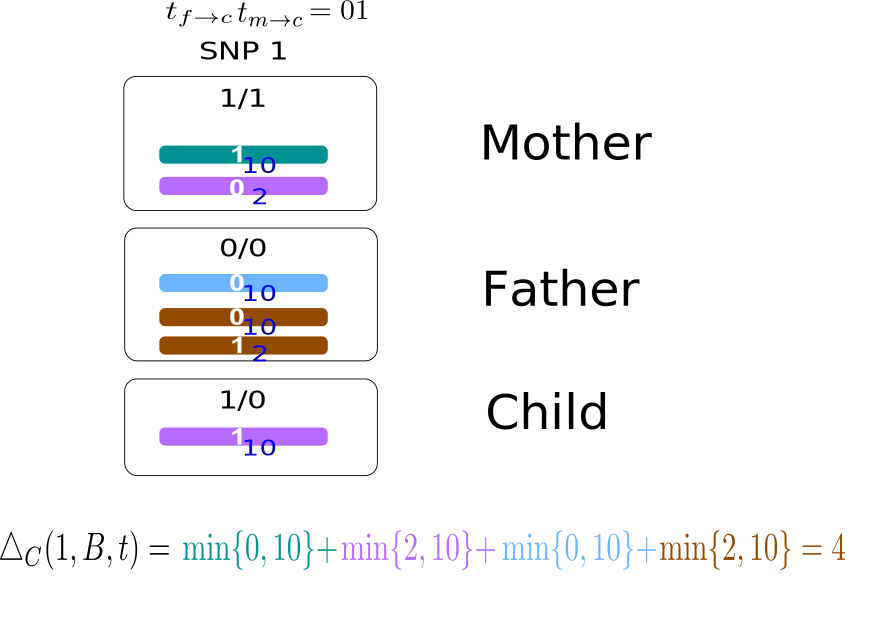
\includegraphics[height=.5\textwidth]{figs/trio-phasing-complete-cost-computation1-second-transmission}
%                                                        % width=0.5\textwidth, height=0.9\textwidth
%							%\end{center}
%
%						\end{column}
%						\vskip5mm
%						 %\vspace*{.1cm}
%						}
%						%\vskip{5mm}
%		\end{columns}
%
%	
%\end{frame}

%\begin{frame}
%	\begin{block}{WhatsHap (Related Individuals)}
%                \scriptsize
%		\textcolor{red}{DP Recurrence}
%		\begin{align}\label{eqn:recurrence}
%			& C(k+1,B,t)= \Delta_C(k+1,B,t)\\
%			& \quad + \min_{\substack{B'\in\mathcal{B}(A(k)):B'\simeq B\\t'\in\{0,1\}^{2 {\mathcal{T}}}}}\big\{C(k,B',t')+d_H(t,t')\cdot\mathcal{X}(k+1)\big\}, \nonumber
%		\end{align}
%	\end{block}
%%	\begin{center}
%\only<1>{		\begin{columns}[]
%			                       \hspace*{10mm}
%
%			\begin{column}{0.4\textwidth}
%				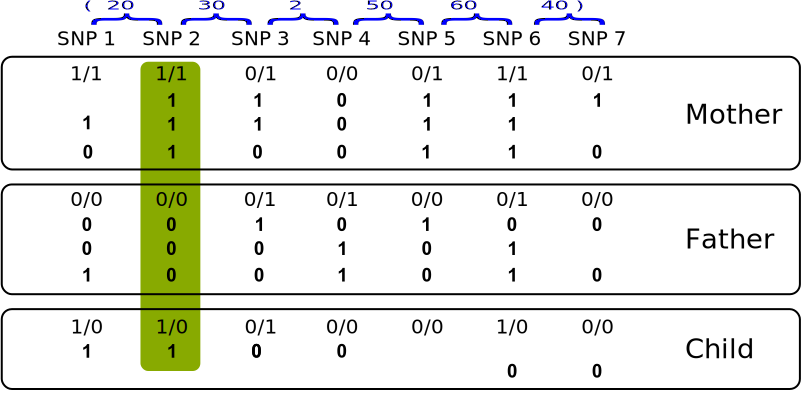
\includegraphics[scale=0.15]{figs/trio-phasing-complete-scond-column}
%                                % width=0.9\textwidth
%				 \begin{block}{}
%				 	\tiny $C(2,B,t)=0+ \min\{4 \ldots        \}$
%				 \end{block}
%
%			\end{column}
%                        \hspace*{2mm}
%			\begin{column}{0.9\textwidth}
%				
%				%\begin{center}
%				%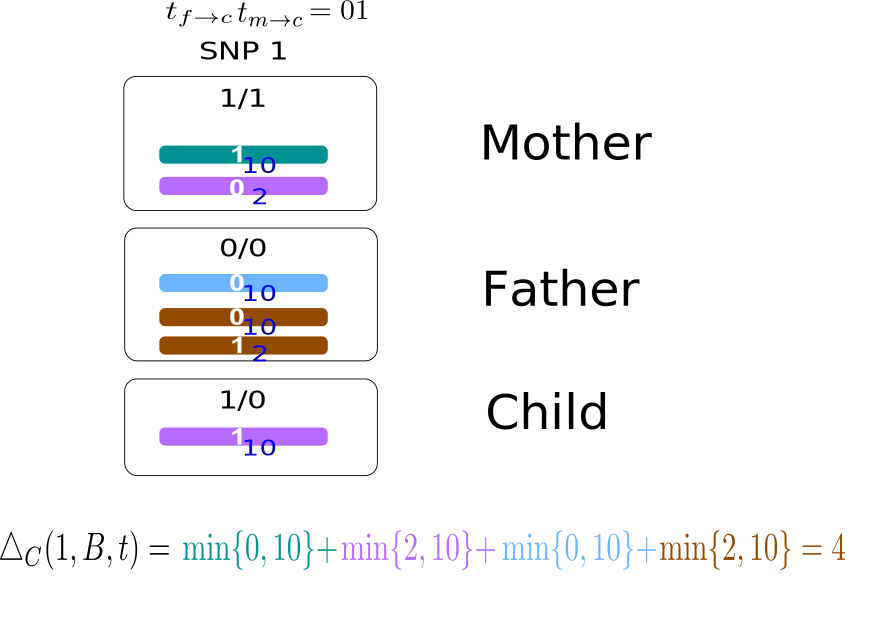
\includegraphics[scale=0.3]{figs/trio-phasing-complete-cost-computation1-second-transmission}
%                                %width=0.5\textwidth, height=0.9\textwidth
%				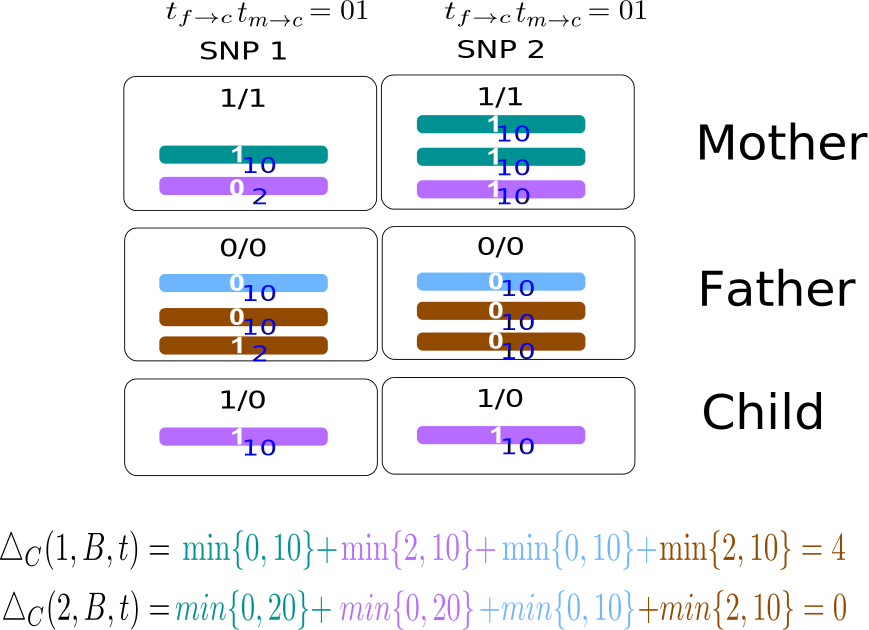
\includegraphics[height=.5\textwidth]{figs/trio-phasing-complete-cost-computation1-second-column-dp-value}\\
%				%\end{center}
%				
%			\end{column}
%		\end{columns}
%	}
%\only<2>{\begin{columns}[]
%	\hspace*{10mm}
%	\begin{column}{0.4\textwidth}
%		\vspace*{1.8mm}
%		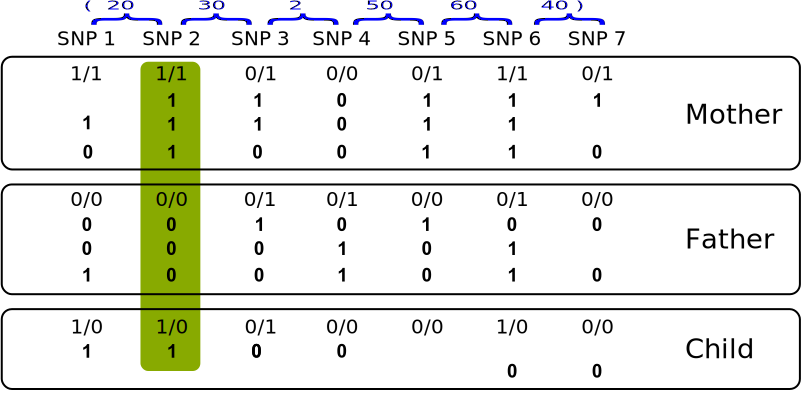
\includegraphics[scale=0.15]{figs/trio-phasing-complete-scond-column}
%		% width=0.9\textwidth
%		\begin{block}{}
%			\tiny $C(2,B,t)=0+ \min\{4, 2 + 1\cdot 20, 4 + 1\cdot 20, 2 + 2\cdot20\}$
%		\end{block}
%		
%	\end{column}
%	\hspace*{2mm}
%	\begin{column}{0.9\textwidth}
%		
%		%\begin{center}
%		%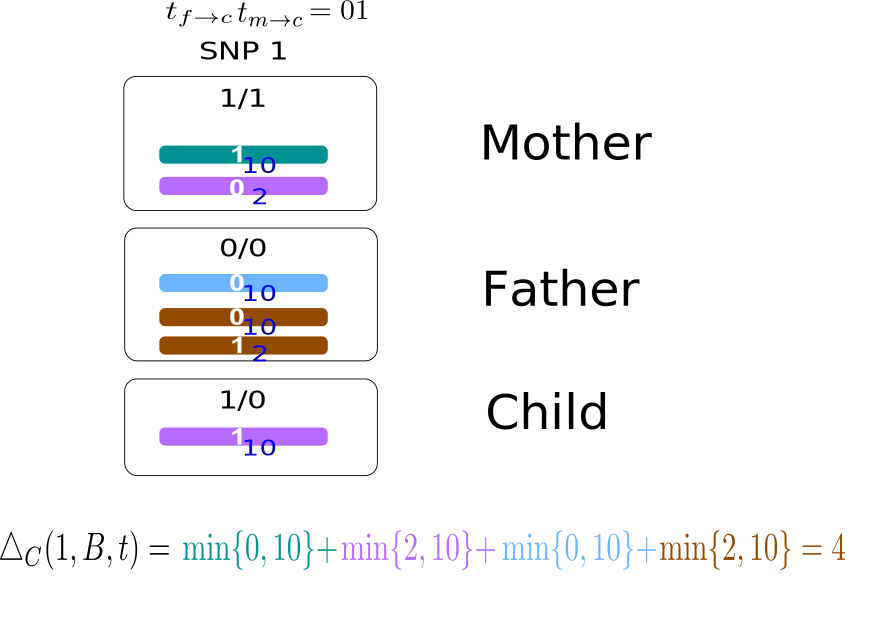
\includegraphics[scale=0.3]{figs/trio-phasing-complete-cost-computation1-second-transmission}
%		%width=0.5\textwidth, height=0.9\textwidth
%		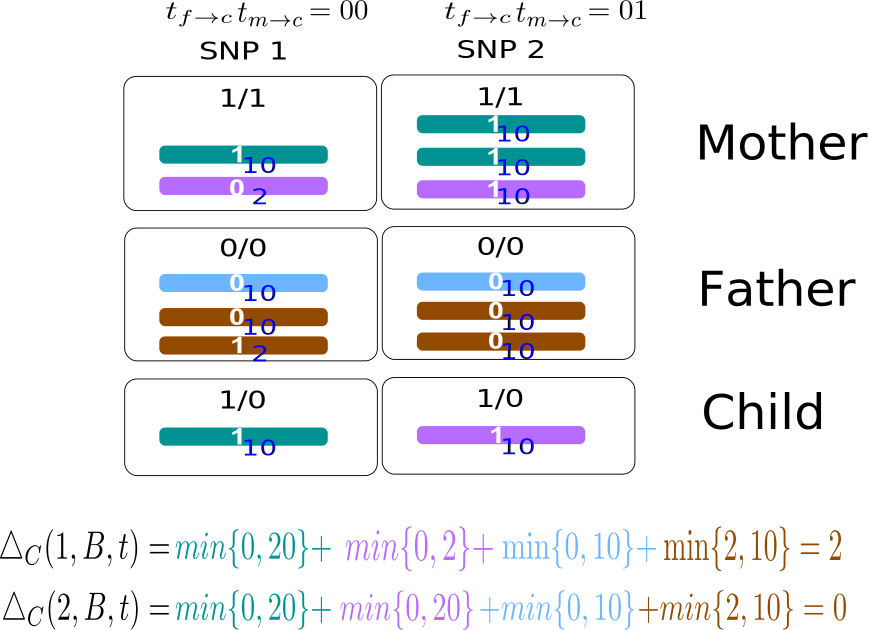
\includegraphics[height=.5\textwidth]{figs/trio-phasing-complete-cost-computation1-second-column-dp-value2}\\
%		%\end{center}
%		
%	\end{column}
%\end{columns}
%	
%	}
%		
%%	\end{center}
%	
%\end{frame}


\begin{frame}{}
	\begin{block}<1->{Runtime}
		Two extra bits for each mother-father-child relationship:
\[O(2^{2t+c}\cdot M)\qquad\qquad\text{(hiding some ugly terms)}\]
		where $c$ is the \emph{maximum of sum of coverages across individuals} and $t$ is the \emph{number of mother-father-child relationship}.
	\end{block}
	\begin{block}<2>{}
		Still feasible for, e.g., $t=1$ and $c=3\cdot 5$. 
		\emph{Linear} in the number of variants.
		\emph{Independent} of read length.
	\end{block}
\end{frame}

%\begin{frame}{Datasets}
%	\begin{itemize}
%		\item \emph{Real Dataset:} AJ trio from Genome in a Bottle Consortium.
%				\begin{itemize}
%					\item \emph{Ground Truth unphased genotypes}
%					\item \emph{Ground Truth phased variants}
%
%					\item PacBio dataset
%					\item 10X Genomics
%				\end{itemize}
%		\item \emph{Simulated Dataset}
%				\begin{itemize}
%					\item Virtual Child
%					\item Simulated PacBio dataset
%				\end{itemize}
%	\end{itemize}
%\end{frame}
\begin{frame}{Datasets}
	\begin{center}
		\includegraphics[scale=0.1]{figs/flowdiagram1}
	\end{center}

\end{frame}

%\begin{frame}
%	\begin{block}{Algorithm: }
%		\textcolor{red}{DP Recurrence}
%		\begin{align}\label{eqn:recurrence}
%		& C(k+1,B,t)= \Delta_C(k+1,B,t)\\
%		& \quad + \min_{\substack{B'\in\mathcal{B}(A(k)):B'\simeq B\\t'\in\{0,1\}^{2\abs{\mathcal{T}}}}}\big\{C(k,B',t')+d_H(t,t')\cdot\mathcal{X}(k+1)\big\}, \nonumber
%		\end{align}
%		\begin{definition}[Bipartition compatibility]
%			Let $B=(P,Q)$ be a bipartition of $A$ and $B'=(P',Q')$ be a bipartition of $A'$.
%			We say that $B$ and $B'$ are \emph{compatible}, written $B\simeq B'$, if
%			$P\cap(A\cap A') = P'\cap(A\cap A')$
%			and
%			$Q\cap(A\cap A') = Q'\cap(A\cap A')$.
%		\end{definition}
%	\end{block}
%		\includegraphics[width=.3\textwidth]{figs/trio-phasing-complete-first-column}
		%\includegraphics[width=.3\textwidth]{figs/trio-phasing-complete-cost-computation1}
%\end{frame}




\begin{frame}{Phasing Related Individuals (Performance)}
\begin{center}
%\only<1>{\includegraphics[scale=.23]{figs/whatshap-pedmec-performance1}} % 
\only<1>{\includegraphics[scale=.23]{figs/whatshap-pedmec-performance2}} %
\only<2>{\includegraphics[scale=.1]{figs/flowdiagram2}} %
\only<3>{\includegraphics[scale=.23]{figs/whatshap-pedmec-performance3}} %
\only<4>{\includegraphics[scale=.1]{figs/flowdiagram}} %
\end{center} %\vspace{-.5em}
%\begin{block}<3>{}
%Note: runtime dominated by reading input files in all cases.
%\end{block}
\end{frame}

\begin{frame}{Comparison to other methods}
\begin{columns}
\begin{column}{.55\textwidth}
\begin{block}{Three \emph{independent} phasings}
\begin{itemize}
 \item PedMEC on 15$\times$ PacBio data
 \item 10xGenomics synthetic long-read phasing
 \item Statistical phasing by SHAPEIT using 1000 Genomes panel
\end{itemize}
\end{block}
\end{column}
\begin{column}{.45\textwidth}
\begin{center}
\only<1>{\includegraphics[scale=0.23]{figs/giab-threeway-left}}%
%\only<2>{\includegraphics[width=\columnwidth]{figs/giab-threeway-both}}%
\end{center}
\end{column}
\end{columns}
\end{frame}

\begin{frame}{Phasing Across Block Boundaries}

	\begin{columns}[]
			\begin{column}{.1\textwidth}
				
			\end{column}
		\begin{column}{0.8\textwidth}
%\begin{center}
		\includegraphics[height=.8\textwidth, width=10\textwidth, keepaspectratio]{figs/long-haplotypes}
%\end{center}
			
			\end{column}
       \hspace*{-2.5cm}
	\begin{column}{.48\textwidth}
			\begin{block}{}
				\emph{Block} is connected component of reads.
				
			\end{block}
	\begin{block}{}
			\begin{itemize}
				\item Phase $99\%$ of the total heterozygous SNPs.
				\item Phasing error rate of $1\%$.
			\end{itemize}
			
		\end{block}
		
	\end{column}
	\begin{column}{\textwidth}

	\end{column}
		\end{columns}
%	\begin{center}
	
%	\end{center}
%	\begin{block}{}
	
%		\begin{itemize}
%			\item Previous slide: no connection by read $\rightarrow$ count as \emph{unphased}
%			\item But there is information \emph{across block boundaries:}
%			\begin{itemize}
%				%\item Phase \emph{between} blocks ``guessed'' correctly in 90\% of all cases.
%				\item Phase $99\%$ of the total heterozygous SNPs in the largest block.
%				\item Phasing error rate of $1\%$.
%			\end{itemize}
%		\end{itemize}
%	\end{block}
\end{frame}

\begin{frame}{Conclusion}
	\begin{itemize}
		\item Formalization of PedMEC problem. 
		\item Unified framework for integrative read-based phasing and genetic haplotyping.
		\item More accurate and complete phasing with family relationship at low coverages of $2\times$ as compared to single individual at $15\times$.
		\item Produces chromosome-length haplotypes by merging the blocks.
		\item \emph{Future plan} is to integrate statistical, genetic and read-based phasing.
	\end{itemize}
	\begin{block}{}
		\emph{Technology Track talk} by Marcel on WhatsHap software on Tuesday at 2:20 pm in the room Northern Hemisphere E3/E4
	\end{block}
\end{frame}

\captionslide{Efficient approach for statistical and read-based phasing}

\begin{frame}{Workflow}
	\begin{center}
		\only<1>{\includegraphics[width=\textwidth, height=175]{figs/pipeline}}%
	\end{center}
\end{frame}





\end{document}
